%
% main.tex -- Paper zum Thema Datenassimilation für Lorenz-System
%
% (c) 2018 Hochschule Rapperswil
%
\chapter{Datenassimilation für das Lorenz-System\label{chapter:kalman}}
\lhead{Datenassimilation für das Lorenz-System}
\begin{refsection}
\chapterauthor{Michael Müller}

\section{Datenassimilation}
\rhead{Datenassimilation}
Die meteorologische Datenassimilation hat zur Aufgabe, Anfangszust"ande f"ur die numerische Wettervorhersage (analysis or filtering mode), Klimaprojektionen (forecasting or predicting mode) oder Untersuchungen am vergangenen Erdklima (reanalysis or smoothing mode) zur Verf"ugung zu stellen, die r"aumlich und zeitlich unvollst"andig vorliegen. Die Datenassimilation nutzt hierzu direkte und indirekte Messungen der Atmosph"are in Kombination mit berechneten Modellzust"anden, um daraus einen in sich stimmigen Gesamtzustand zu ermitteln. Die Ermittlung des Zustandes der Atmosph"are erfolgt in regelm"assigen zeitlichen Abst"anden, dem sogenannten Datenassimilations-Zyklus, durch welchen eine verl"assliche Bestimmung der atmosph"arischen Gr"ossen wie Druck oder Temperatur m"oglich wird.

\section{Kalmanfilter}
\rhead{Kalmanfilter}
Ein Werkzeug der Datenassimilation ist der Kalmanfilter mit seinen diversen Abwandlungen. In diesem Kapitel wird der Kalmanfilter genauer erkl"art und auf die Parameter eingegangen. Am Lorenzmodell aus dem Jahre 1963 (LM63) kommt eine erweiterte Version zur Anwendung, der sogenannte Extended Kalmanfilter. Dieser ist f"ur nicht-lineare dynamische Systeme erweitert worden und wurde im Zuge der Apollo Mission von Stanley F. Schmidt entwickelt und zur Navigation im Weltraum angewendet\cite{skript:NASAKalman}.

Der Kalmanfilter ist ein rekursives Verfahren zur Filterung von Datens"atzen, bei dem  der zuk"unftige Datenpunkt als Linearkombination der Beobachtung und einer Vorhersage durch ein mathematisches Systemmodell gesch"atzt wird. Voraussetzung f"ur die Beobachtung ist die Messung mindestens einer Systemvariablen mit zugeh"origer Varianz. Im linearen Fall ist f"ur das Modell eine Matrix n"otig, die aus dem alten Zustand auf den neuen schliessen l"asst, wie detaillierter in\cite{skript:WRStat} gezeigt wird.\\

\subsection{Allgemeine Funktionsweise}
\rhead{Allgemeine Funktionsweise}

Die Struktur des Kalmanfilter-Algorithmus erlaubt eine Echtzeitfilterung und macht ihn so f"ur diverse Anwendungen interessant.\\
Folgend ist $\phi \in \mathbb{R}^{n\times n}$ die Transformationsmatrix, $H \in \mathbb{R}^{m\times n}$ die Messmatrix, welche Systemvariablen $x_{k}\in \mathbb{R}^{m}$ mit allf"alliger Verst"arkung misst und woraus $z_{k}\in \mathbb{R}^{m}$ als Messwert resultiert. $R_{k}$ und $Q_{k}$ sind die Kovarianzen der Messung und des Systems und Elemente des $\mathbb{R}^{m\times m}$. Das Systemmodell \eqref{kalman:Simulation} wie auch die Messung \eqref{kalman:Messung} sind mit einem normalverteilten Fehler, $u_{k}$ und $w_{k}$, "uberlagert\cite{skript:WRStat}.

\begin{align}
x_{k}&=\phi_{k-1}x_{k-1}+u_{k} \text{, } &\text{mit } u_{k}\sim N\langle0,\sigma^{2}\rangle &\text{ und } Q_{k}=E(u_{k}u^{t}_{k}) \label{kalman:Simulation}\\
z_{k}&=H_{k}x_{k}+w_{k} \text{ ,} &\text{mit } w_{k}\sim N\langle0,\sigma^{2}\rangle &\text{ und } R_{k}=E(w_{k}w^{t}_{k})
\label{kalman:Messung}
\end{align}


Der Algorithmus besteht aus folgender Schrittfolge:
\begin{enumerate}

\item Vorhersage\\
Die Vorhersage wird sowohl f"ur den folgenden Datenpunkt $\hat{x}_{k+1|k}$ sowie dessen Kovarianz $P \in \mathbb{R}^{m\times m}$ durchgef"uhrt, wobei das $\phi$ die Transformationsmatrix ausdr"uckt, wie vom jetzigen Zustand auf den n"achsten geschlossen wird. Die Notation $\hat{x}_{k+1|k}$ bedeutet die Sch"atzung von $x$ zum Zeitpunkt $k$ f"ur den n"achsten Zeitpunkt $k+1$ .

\begin{align*}
\hat{x}_{k+1|k} &= \phi\hat{x}_{k}\\
P_{k+1|k} &=\phi_{k}P_{k}\phi_{k}^{t}+Q_{k}
\end{align*}

\item Kalmanfaktor\\
Der Kalmanfaktor $K \in \mathbb{R}^{n\times n}$, gewichtet in Abh"angigkeit der beiden Fehlerkovarianzen die Beobachtung oder das Systemmodell st"arker. Dabei l"ost der Algorithmus das Problem optimal, so dass sich f"ur die sp"ater korrigierte Vorhersage das Minimum der resultierenden Kovarianz ergibt.\\
\[K_{k}=P_{k|k-1}H^{t}_{k}(H_{k}P_{k|k-1}H^{t}_{k}+R_{k})^{-1}   \]

\item Korrektur\\
Die Vorhersage wird nun mit dem Kalmanfaktor und der Messung korrigiert. In der folgenden Beschreibung ist die Gewichtung durch den Kalmanfaktor in der Matrixschreibweise zu erkennen. Dasselbe Vorgehen gilt f"ur die Kovarianzmatrix $P$.

\begin{align*}
\hat{x}_{k}&=(I-K_{k}H_{k})\hat{x}_{k|k-1}+K_{k}z_{k} \\
P_{k} &=(I-K_{k}H_{k})P_{k|k-1}(I-K_{k}H_{k})^{t}+K_{k}R_{k}K^{t}_{k}  \end{align*}
\end{enumerate}

\subsection{Anwendung auf das Lorenz-System}
\rhead{Anwendung auf das Lorenz-System}
Nun die Anwendung des Kalmanfilter auf das LM63, mit dem folgenden ber"uhmten Differentialgleichungssystems.
\begin{align}
\dot x &= -\sigma x + \sigma y\\
\dot y &= \varrho x - y - x z\\
\dot z &= -\beta z + x y
\label{kalman:lm63} 
\end{align}

\subsubsection{Systemmodellierung}
\rhead{Systemmodellierung}
Als erstes ist f"ur die Vorhersage die Transformationsmatrix $\phi$ notwendig, dessen Herleitung und Gebrauch n"ahere Erl"auterungen ben"otigt. Deshalb als Einf"uhrung ein einfacheres Beispiel aus der translatorischen Bewegungsgleichung \eqref{kalman:Posbest} zur Positionsbestimmung, wie sie beispielsweise bei autonomen Fahrzeugen zum Einsatz kommt.

\begin{align}
\underbrace{\begin{pmatrix}
s_{k+1|k} \\ 
v_{k+1|k} \\ 
a_{k+1|k}
\end{pmatrix}}_{\hat{x}_{k+1}}
&=
\underbrace{\begin{pmatrix}
 1 & \Delta t & \frac{1}{2}\Delta t^{2} \\ 
 0 & 1 & \Delta t \\ 
 0 & 0 & 1
 \end{pmatrix}}_{\phi}
\underbrace{\begin{pmatrix}
   s_{k} \\ 
   v_{k} \\ 
   a_{k}
   \end{pmatrix}}_{\hat{x}_{k}}
\label{kalman:Posbest}
\end{align}
Die Matrix $\phi$ f"ur das nicht-lineare System, wie das LM63, kann nicht auf diese  Weise aufgestellt werden. Eine M"oglichkeit ist die Abh"angigkeit von Anfangsbedingungen, daher wie stark "andert sich der Zielwert, wenn die Anfangsbedingung(en) um ein $\Delta x_{0}$ ver"andert wird. Abbildung \ref{kalman:AblnachAnf} zeigt einen Ausschnitt aus dem Lorenzmodell, wo die Anfangsbedingungen gegen"uber dem 'Original' in rot zum Zeitpunkt $k$ geringf"uging ver"andert wurde und welche Auswirkung dies, innerhalb eines Zykluses, auf den nächsten Datenpunkt $k+1$ hat.

\begin{figure}
\centering
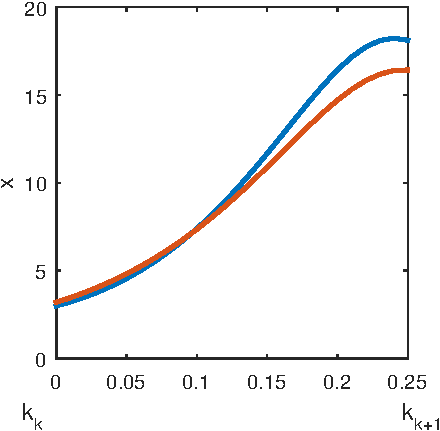
\includegraphics[width=3in]{kalman/figures/ablnachAnf2.pdf}
\caption{Auschnitt der $x$-Koordinate des LM63: Ver"anderung der Anfangsbedingungen zum Zeitpunkt $k$ und Auswirkung bei $k+1$}
\label{kalman:AblnachAnf}
\end{figure}

W"ahrend des Datenassimilations-Zyklus wird das Systemmodell mit den Anfangsbedingungen sowie dem $\phi$ mittels der Formel
\[
\frac{d}{dt}\begin{pmatrix}
x \\ 
y \\ 
z \\ 
\textbf{J}
\end{pmatrix}=
\begin{pmatrix}
f(x,y,z) \\ 
\textbf{F}(x,y,z)\textbf{J}
\end{pmatrix} 
\text{, mit Anfangsbedingung }
x(0)=\begin{pmatrix}
x_{0}\\
y_{0}\\
z_{0}\\ 
\textbf{E}
\end{pmatrix} 
\]
gel"ost und integriert, wobei $F$ die Jakobische Matrix des LM63 
\[
F(x,y,z) = \begin{pmatrix}
-\sigma & \sigma & 0 \\ 
\rho-z & -1 & -x \\ 
y & x & -\beta
\end{pmatrix} 
\]
ist. \textbf{J} und \textbf{E} sind $3\times3$ Matrizen, die spaltenweise in den Vektor eingef"ullt wurden. $f(x,y,z)$ ist die rechte Seite des LM63 gem"ass Formel \eqref{kalman:lm63}. Der gel"oste Vektor hat dann f"ur unser System folgende Form.
\[
x_{k}=\begin{pmatrix}
x \\ 
y \\ 
z \\  
J_{11} \\ 
J_{12} \\ 
J_{13} \\ 
J_{21} \\ 
J_{22} \\ 
J_{23} \\ 
J_{31} \\ 
J_{32} \\
J_{33} 
\end{pmatrix}
\]
Die letzten 9 Eintr"age aus $x_{k}$ werden nun wieder spaltenweise in eine 3x3 Matrix umgewandelt, welche nun unser gesuchtes $\phi$ ist. Die drei ersten Eintr"age sind die L"osung des Lorenzmodells als Zwischenschritte w"ahrend des Datenassimilationszyklus, welche sp"ater als blaue Kreuze dargestellt werden. Die Herleitung und weitere Erl"auterungen zum Vorgehen sind in \cite{skript:DiffGl} zu finden.\\

\subsubsection{Messystem}
\rhead{Messsystem}
Die Messmatrizen, die f"ur diese Arbeit Verwendung finden, sind folgende:
\[H_{1}=\begin{pmatrix}
1 & 0 & 0 \\ 
0 & 1 & 0 \\ 
0 & 0 & 1
\end{pmatrix} 
\text{, }
H_{2}=\begin{pmatrix}
1 & 1 & 0 \\ 
0 & 1 & 1 \\ 
\end{pmatrix}
\text{, }
H_{3}=\begin{pmatrix}
1 & 0 & 0 \\ 
0 & 1 & 0 \\ 
\end{pmatrix}
\text{, }
H_{4}=\begin{pmatrix}
1 & 0 & 0 \\  
0 & 0 & 1
\end{pmatrix}
\]
Die Einheitsmatrix $H_{1}$ misst zum Beispiel jeden der drei Eintr"age des Lorenz Systems
\[
\begin{pmatrix}
x\\
y\\
z
\end{pmatrix}
\text{.}
\]
Die zweite Messmatrix misst den $x$-Eintrag nur als Kombination von $x$ und $y$ sowie den $y$-Eintrag als Kombination von $y$ und $z$, was oft die Realit"at widerspiegelt, wo Messgr"ossen nicht direkt gemessen werden k"onnen. $H_{3}$ und $H_{4}$ als anspruchsvolle Beispiele f"ur den Filter, wo Messwerte fehlen und damit f"ur je eine Variable keine Korrekturm"oglichkeit besteht.

Der Messwert mit $H_{3}$ sieht dann zum Beispiel wie folgt aus:
\[\hat{z}_{k}=
\begin{pmatrix}
\hat{x} \\
\hat{y} \\
\end{pmatrix}= 
\underbrace{\begin{pmatrix}
1 & 0 & 0  \\
0 & 1 & 0
\end{pmatrix}}_{H_{3}}
\underbrace{\begin{pmatrix}
x \\
y \\
z \\
\end{pmatrix}
}_{x_{k}}
+
\underbrace{\begin{pmatrix}
\sigma_{x} & 0 \\
0 & \sigma_{y}
\end{pmatrix}}_{\text{Fehler R}}
\]

\subsubsection{Fehlermodellierung}
\rhead{Fehlermodellierung}
Weitere wichtige Parameter des Filters sind die Fehlerkovarianzen, sie sind konstant und haben bei vollst"andig erfassbarem Messsystem folgende Form.
\[R=\begin{pmatrix}
\sigma^{2}_{x} & 0 & 0 \\ 
0 & \sigma^{2}_{y} & 0 \\ 
0 & 0 & \sigma^{2}_{z}
\end{pmatrix}  \text{,}\qquad
Q=\begin{pmatrix}
\sigma^{2}_{x} & 0 & 0 \\ 
0 & \sigma^{2}_{y} & 0 \\ 
0 & 0 & \sigma^{2}_{z}
\end{pmatrix} 
\]

\subsection{Parameter und Initialisierung}
\rhead{Parameter und Initialisierung}
Die Werte f"ur die charakteristischen Parameter des Lorenz-System, unter denen das chaotisches Verhalten auftritt, werden auch hier verwendet. Es gilt $\sigma=10$, $\beta=8/3$ und $\rho=28$. Der Startwert
\[
x_{0}=\begin{pmatrix}
3 \\ 
5 \\ 
5
\end{pmatrix}
\]
ist vom Standardwert
\[
x_{0,Standard}=
\begin{pmatrix}
3\\
15\\
1
\end{pmatrix}\]
verschieden, um das chaotische Verhalten schneller herbeizuf"uhren und Rechenzeit einzusparen. Gezeigt wird auch nur jeweils der Ausschnitt $t = [5,10]$, da an der Stelle das chaotische Verhalten ausgepr"agt vorhanden ist. 
Die Initialisierung von
\[
P_{0}=\begin{pmatrix}
10 & 0 & 0 \\ 
0 & 10 & 0 \\ 
0 & 0 & 10
\end{pmatrix}
\]
f"ur die Varianz der Simulation, ist zur Sicherheit gross gew"ahlt. Dies hat f"ur die Berechnung keinen signifikanten Einfluss, da der Algorithmus den Wert zeitnah korrigiert. $J$ wird mit der Einheitsmatrix
\[
\begin{pmatrix}
1 & 0 & 0 \\ 
0 & 1 & 0 \\ 
0 & 0 & 1
\end{pmatrix} 
\]
initialisiert und dient der Berechnung des $\phi$. Diese Matrix wird "uber mehrere Zwischenschritte, mit Vorhersage und Korrektur, bis zum Zeitpunkt $t_{k+1}$ integriert.

Zuf"allige St"orsignale in der Messung oder in die Simulation werden keine eingebaut, da aufgrund der starken Vereinfachungen und Transformationen bis hin zum Lorenzmodell aus einem urspr"unglichen Messfehler (z.B. $\pm1^\circ C$) ohnehin kein R"uckschluss auf Abweichungen im Modell mehr m"oglich w"are.


\subsection{Die Realit"at}
\rhead{Die Realit"at}
Das Ziel bleibt, den Zustand eines Wetter- oder Klimasystems zu sch"atzen oder gar vorhersagen zu k"onnen. Da ein vollst"andiges und korrektes Modell nicht zur Verf"ugung steht, begn"ugen wir uns mit dem gegebenen LM63. Dieses System ist einfach genug, damit wir mit den genannten Parametern eine virtuelle Realit"at durch L"osen des Differentialgleichungssystems erzeugen k"onnen. Die Wetter- und Klimabeobachtung erlaubt uns nicht, alle Parameter mit beliebiger Genauigkeit zu bestimmen, unsere Messungen sind immer unvollst"andig und mit Fehlern behaftet. Wir versuchen aber, den tats"achlichen Zustand des Systems, also die berechnete Realit"at aus fehlerbehaften Messungen zu rekonstruieren.

In Abbildung \ref{kalman:Oberfl} sind alle Ansichten wie das 3D Modell und die Ansicht jeder Koordinate zusammengetragen, die f"ur die Untersuchungen notwendig sind.

Die roten Linien sind jeweils unsere erzeugte Realit"at, die blauen Sterne die simulierten Vorhersagen w"ahrend des Datenassimilationszyklus und die roten Kreise die gefilterten Werte. Die Grafik zeigt auch, das trotz sehr genauer Messung und folglich einer marginalen Abweichung vom Anfangszustand eine Vorhersage nur f"ur einen beschr"ankten Zeitraum m"oglich ist. 

\begin{figure}
\centering
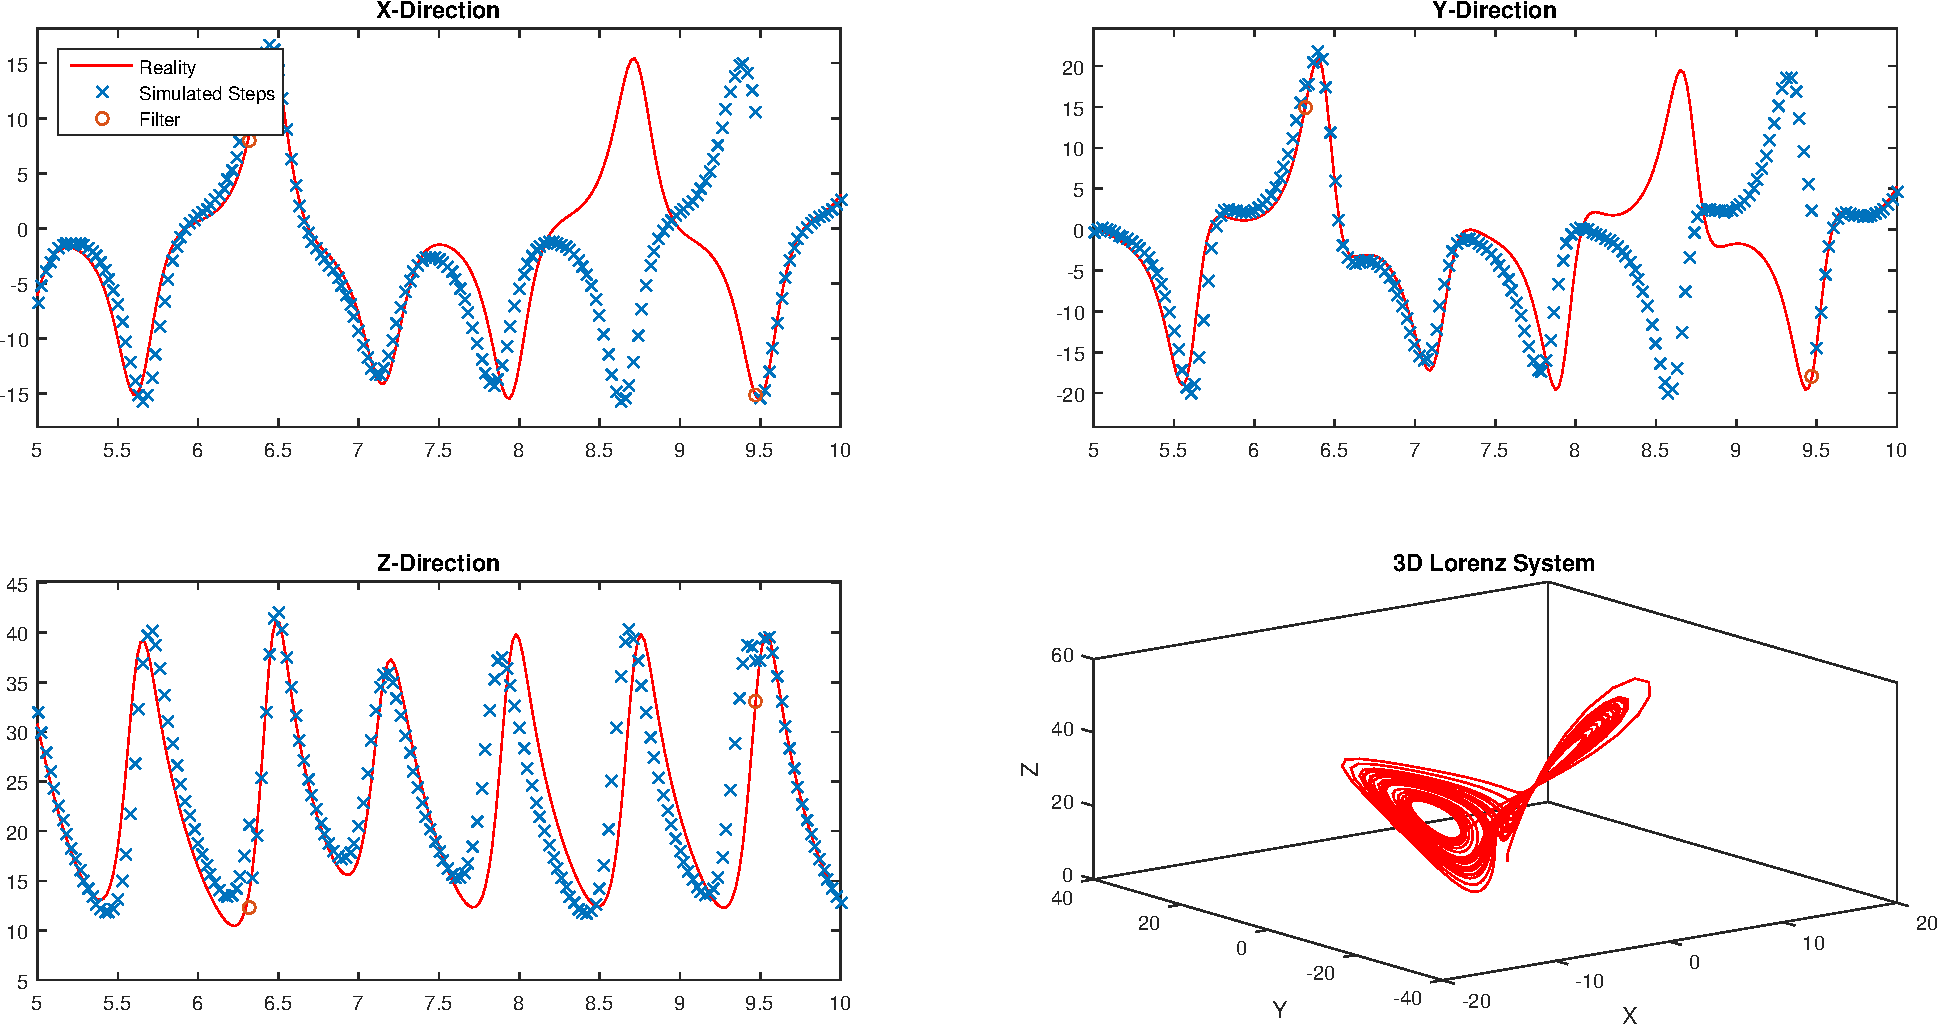
\includegraphics[width=\hsize]{kalman/figures/3dsystemview.pdf}
\caption{Beispielhafte Darstellung der drei Achsansichten mit Legende und als 3-D Plot}
\label{kalman:Oberfl}
\end{figure}

\subsection{Anmerkungen zur Kovarianzmatrix und dem Kalmanfaktor}
\rhead{Anmerkungen zur Kovarianzmatrix und dem Kalmanfaktor}
Im Falle der Positionsbestimmung \eqref{kalman:Posbest} sind
\begin{align*}
P_{k+1|k}&=f(\phi, Q)\\
K&=f(P,H,R)\\
P_{k}&=f(K,H,R)
\end{align*}
Konstanten,da alle Parameter ebenfalls konstant sind. So m"ussen sie nicht in jedem Datenassimilations-Zyklus neu berechnet werden und k"onnen, nach einmaliger Berechnung, als Konstanten einprogrammiert werden. Im Falle des LM63 ist das $\phi$ variabel, weshalb $K$ und $P$ auch variabel sind und jeweils berechnet werden m"ussen. Zwei Beispiele sind in der Abbildung \ref{kalman:Kovarianz} dargestellt. Es ist sowohl eine deutliche Abnahme der Genauigkeit $P$ sowie eine st"arkere Fluktuationen von der Messmatrix $H_{1}$ zu $H_{2}$ zu erkennen.

\begin{figure}
\centering
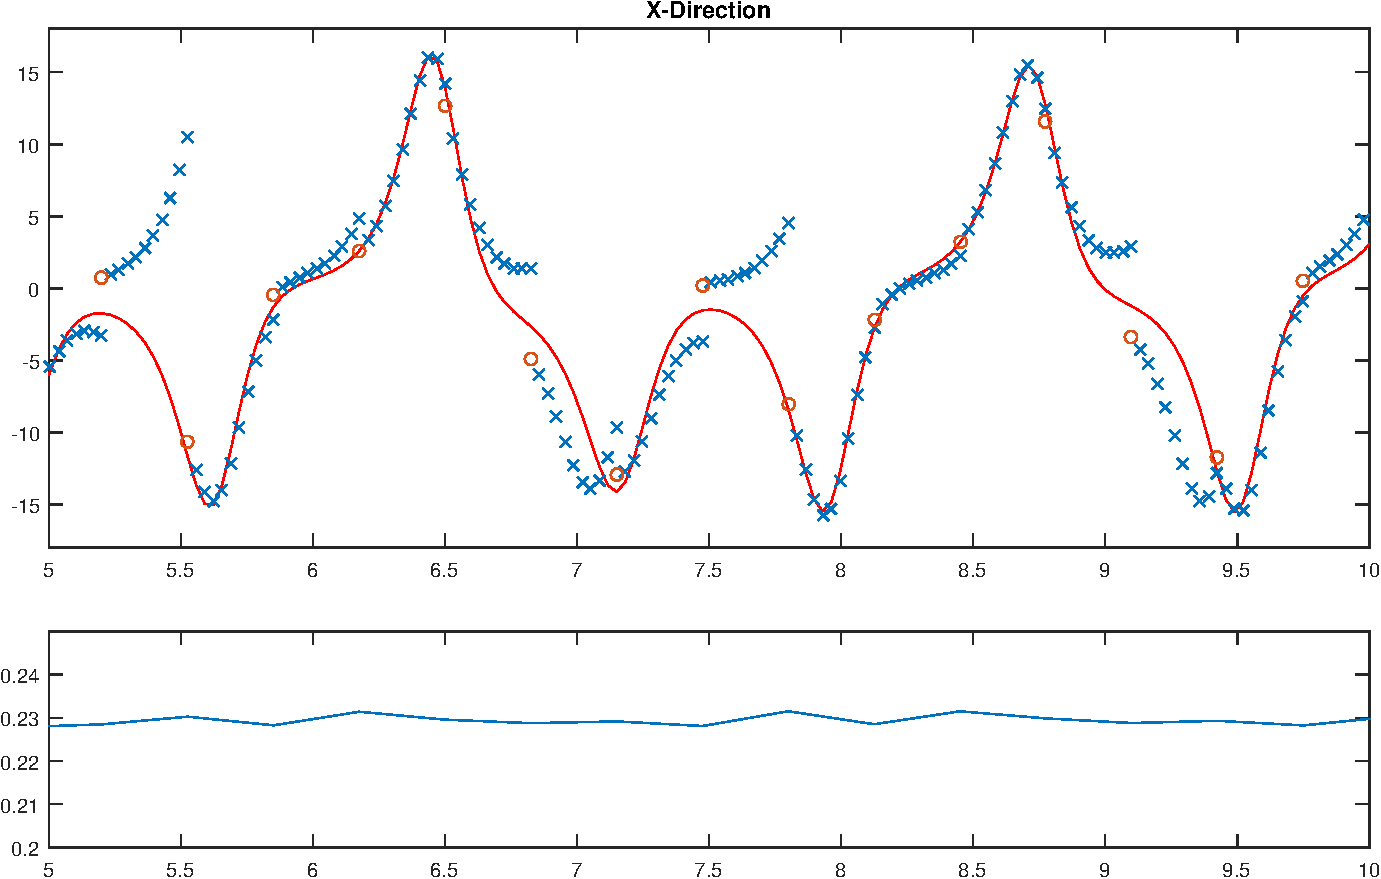
\includegraphics[width=\hsize]{kalman/figures/H1R10S2XP.pdf}
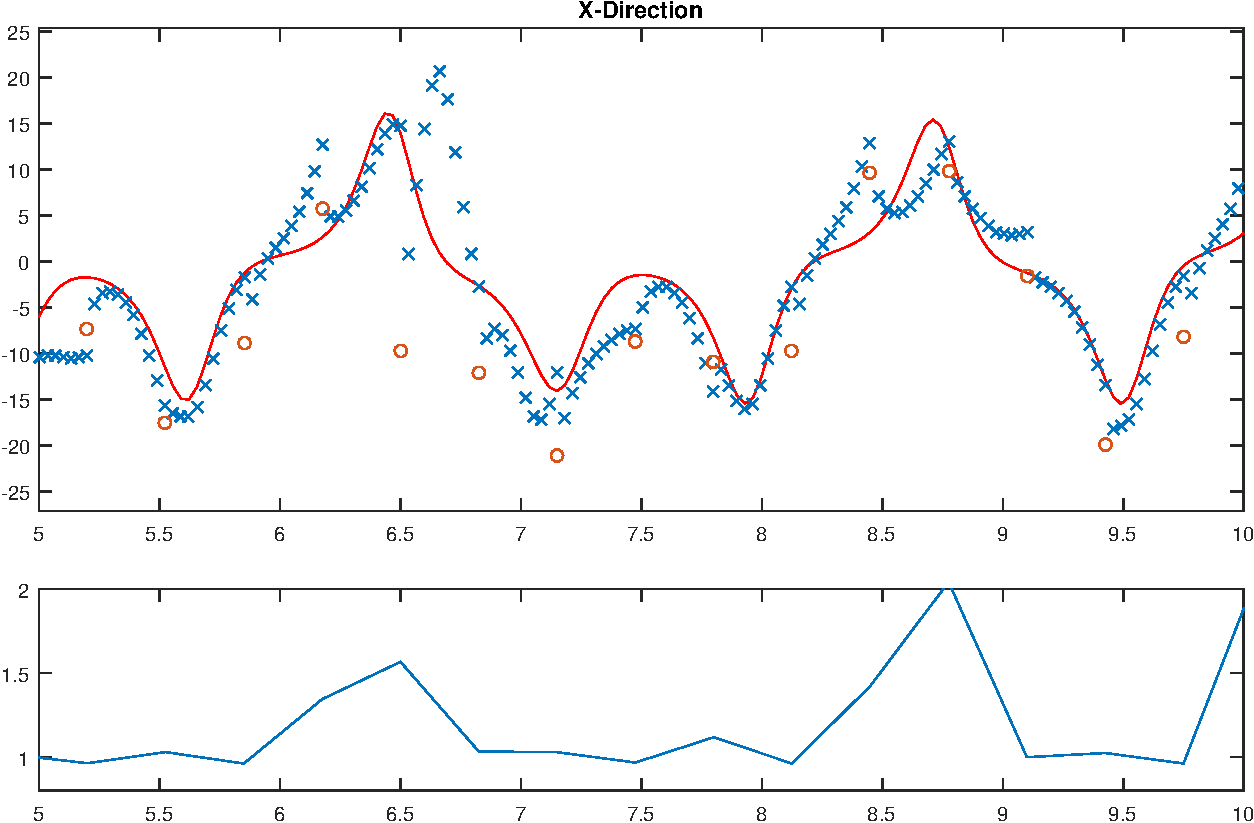
\includegraphics[width=\hsize]{kalman/figures/H2R10S2XP.pdf}
\caption{Filteroutput f"ur die X-Achse mit Kovarianzmatrix $P_{11}$ bei direkter Messung mit $H_{1}$ der Zustandsvariablen (oben) und bei indirekter Messung mit $H_{2}$ (unten)}
\label{kalman:Kovarianz}
\end{figure}

\section{Beobachtungen und Erkenntnisse}
\rhead{Beobachtungen und Erkenntnisse}
In diesem Kapitel werden aufgestellte Hypothesen besprochen und mit Simulationen verdeutlicht. Das LM63 wird mit den vorgestellten Messmatritzen gemessen und gefiltert. Um die Anzahl Variablen zu reduzieren, wird die dimensionslose Gr"osse
\[
F=\frac{Q}{R}
\]
verwendet. Ein $F>1$ bedeutet, dass die Messung genauer ist, als die simulierte Vorhersage, sodass diese st"arker gewichtet wird. Die absolute Fehlervarianz ist f"ur den Filteralgorithmus irrelevant, da lediglich das Verh"altnis Einfluss auf die Gewichtung nimmt.

Um den Datenassimilations-Zyklus dimensionslos darzustellen, bildet $S$ die Schrittmenge pro Oszillation. Trotz der chaotischen Oszillation in zwei Richtungen ist diese nahezu konstant. Gilt zum Beispiel $S=2$, so werden pro Oszillation zwei Messungen durchgef"uhrt. Da diese nicht konstant ist, erfolgen die Messungen nicht immer am selben Ort.

\subsection{Vollst"andig erfassbares System}
\rhead{Vollst"andig erfassberes System}
Als vollst"andig erfassbares System gelten hier die Systeme mit den Messmatritzen
\[
H_{1}=\begin{pmatrix}
1 & 0 & 0 \\ 
0 & 1 & 0 \\ 
0 & 0 & 1
\end{pmatrix} 
\text{ und }
H_{2}=\begin{pmatrix}
1 & 1 & 0 \\ 
0 & 1 & 1 \\ 
\end{pmatrix}
\text{.}
\]
Eine naheliegende Vermutung ist, dass eine genauere Messung, bessere Vorhersagen "uber einen l"angeren Zeitraum erlaubt. Also aus einem gr"osseren $F$ resultieren besser Vorhersagen, was die oberen beiden Bilder in Abbildung \ref{kalman:H1S1} illustrieren. Dies gilt aber nur, wenn das Systemmodell gut mit der Realit"at korreliert, was in diesem Versuch der Fall ist, da die Realit"at genau dem Systemmodell entspricht.
Was ein Vergleich der unteren Bilder deutlich zeigt, ist dass der Mehraufwand an Messgenauigkeit auch dadurch kompensiert werden kann, in dem zu einem g"unstigerem Zeitpunkt gemessen wird. Hierbei zeigt sich deutlich das Chaos des System, wo nicht quantitativ beurteilt werden kann, zu welchen Zeitpunkt welche Genauigkeiten notwendig sind.
\begin{figure}
\centering
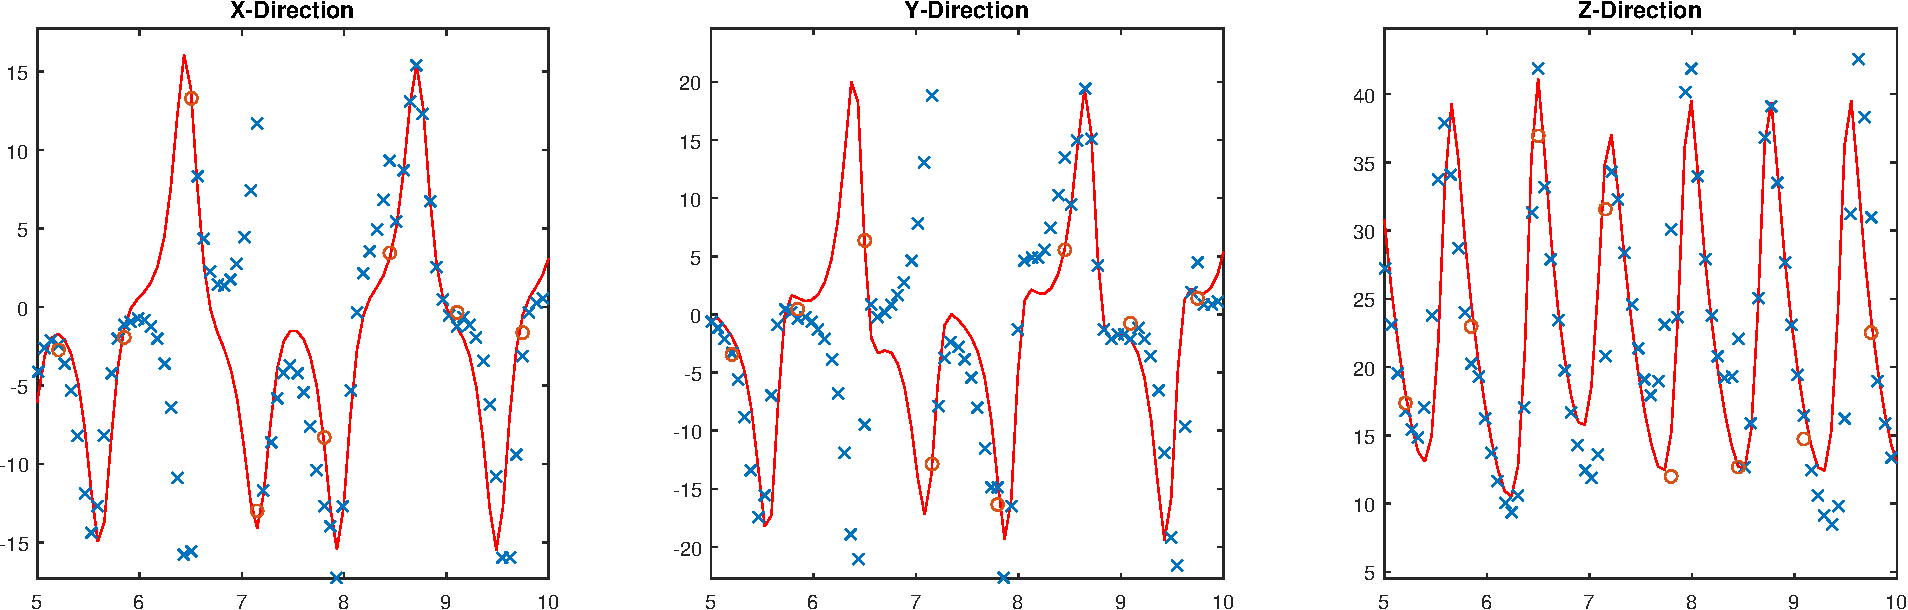
\includegraphics[width=\hsize]{kalman/figures/H1R10S1.pdf}
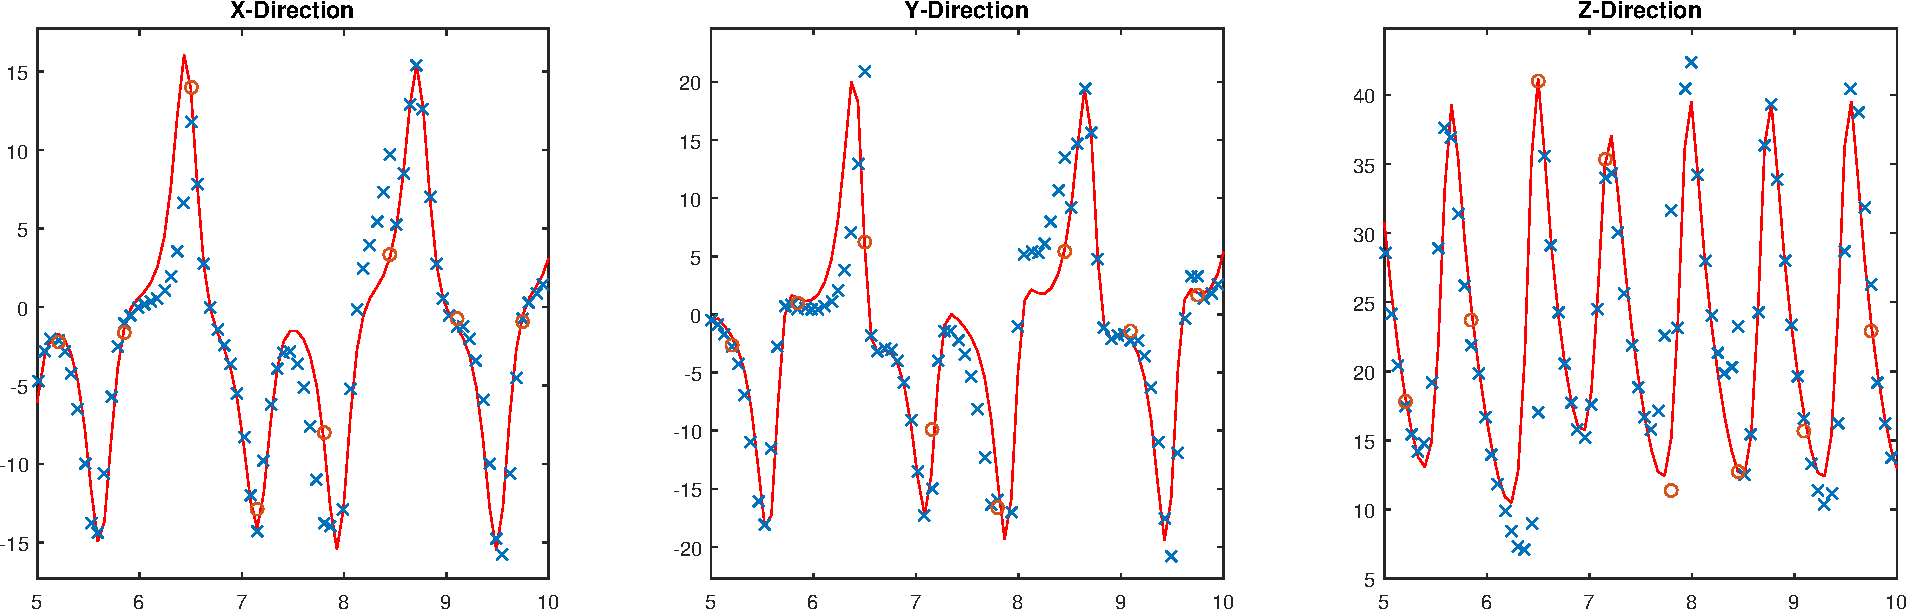
\includegraphics[width=\hsize]{kalman/figures/H1R20S1.pdf}
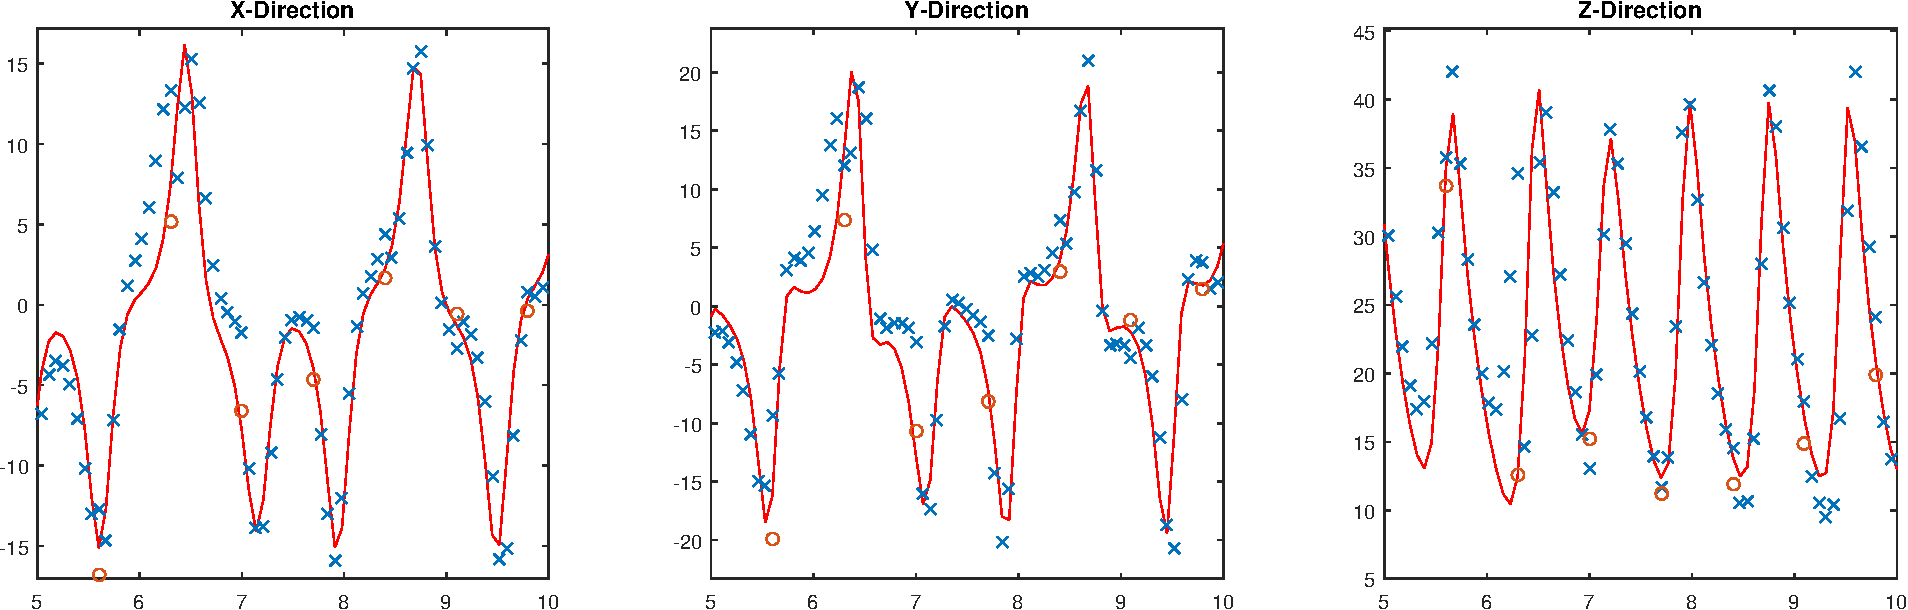
\includegraphics[width=\hsize]{kalman/figures/H1R10S1aS.pdf}
\caption{Messmatrix $H_{1}$ jeweils mit $S=1$ und $F=10$ (oben), $F=20$ (mitte) und $F=10$ (unten), letztere mit versetzter Messung}
\label{kalman:H1S1}
\end{figure}

Abbildung \ref{kalman:H1S2} zeigt das Modell in dem Messungen zweimal pro Oszillation zur Verf"ugung stehen. So steht eine korrigierende Messung schneller zur Verf"ugung, jedoch wird auch der Vorhersage-Zeitraum k"urzer, was denn Zweck des Filters zunehmend einschr"ankt. Deutliche Verbesserungen gegen"uber vorhin sind nicht zu erkennen, sie werden in diesem Beispiel sogar schlechter. Je h"aufiger das gemessen wird, desto weniger relevant wird zudem der Zeitpunkt der Messung.
Um die Relevanz nochmals zu verdeutlichen, eine Vorhersage in die entgegengesetzte Richtung bedeutet, dass die Drehrichtung  der Konvektionsstr"ome falsch gesch"atzt wurde.
\begin{figure}
\centering
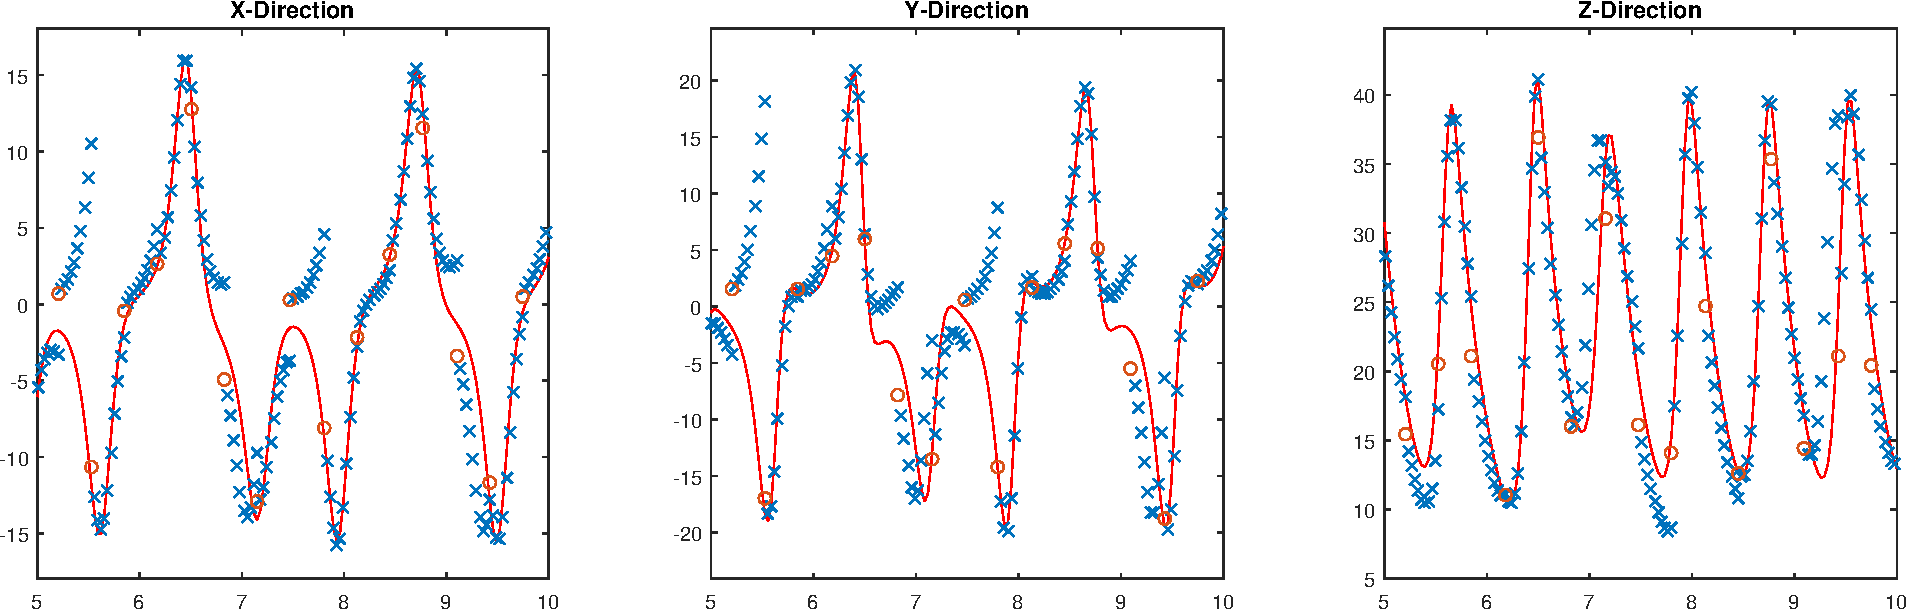
\includegraphics[width=\hsize]{kalman/figures/H1R10S2.pdf}
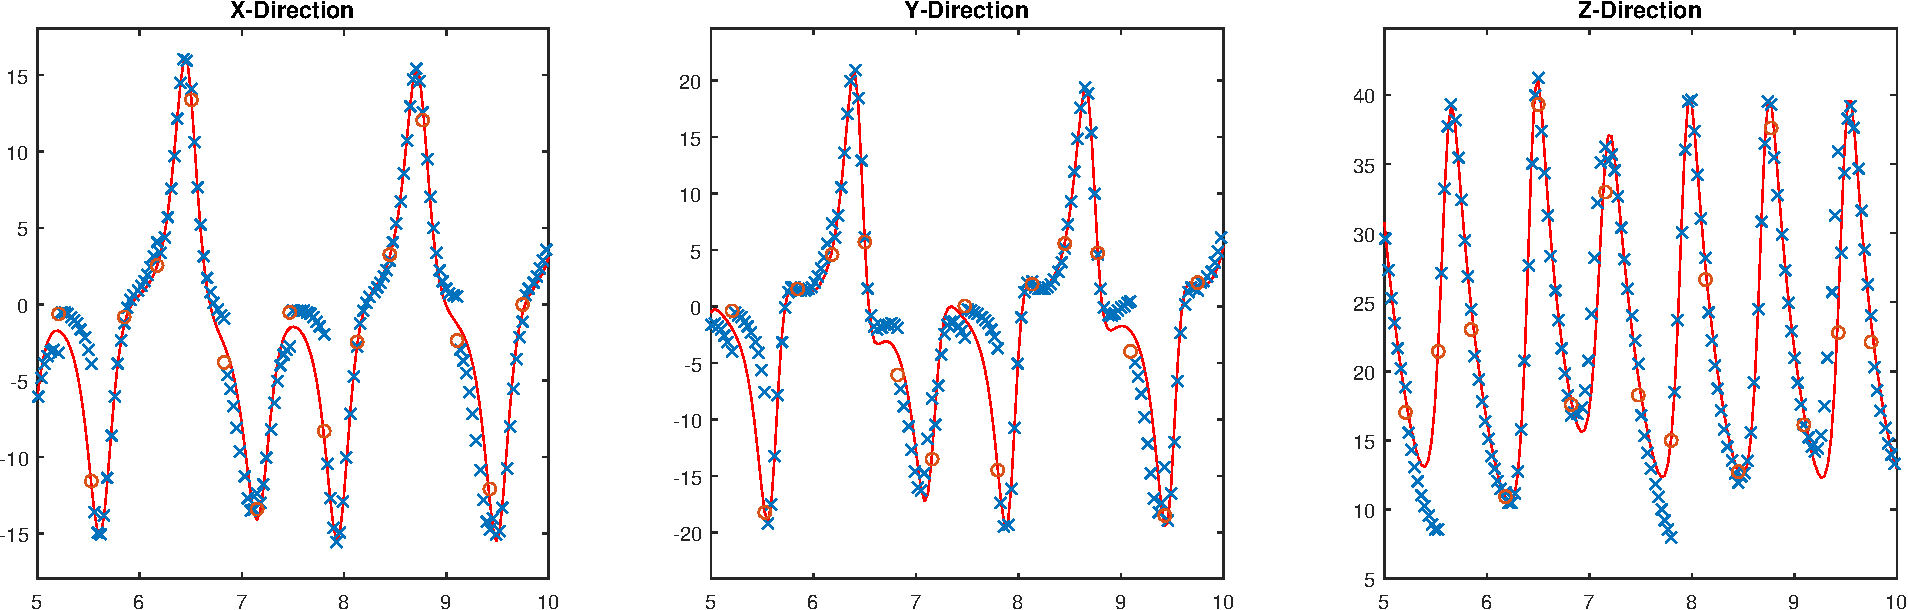
\includegraphics[width=\hsize]{kalman/figures/H1R25S2.pdf}
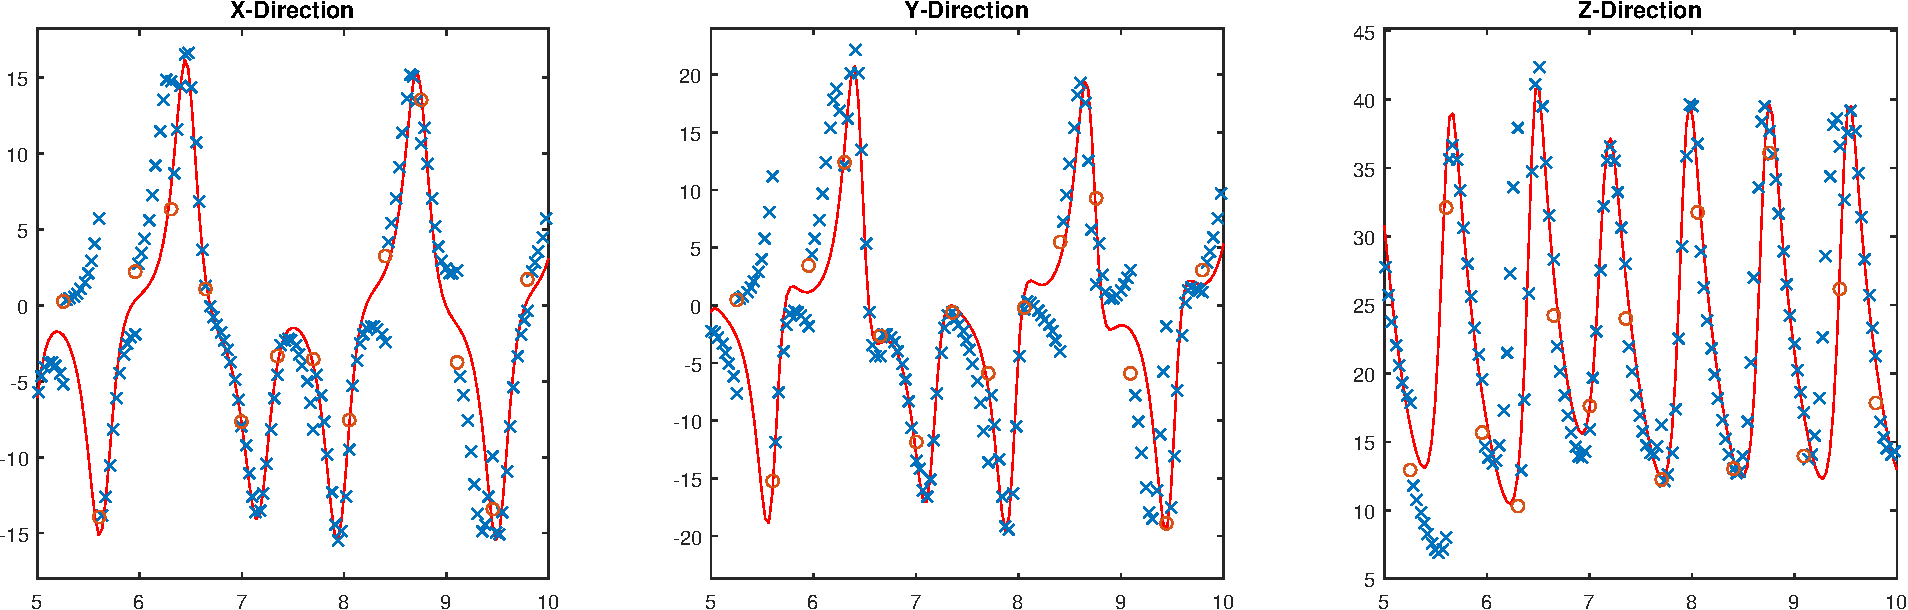
\includegraphics[width=\hsize]{kalman/figures/H1R10S2aS.pdf}
\caption{Messmatrix $H_{1}$ jeweils mit $S=2$ und $F=10$ (oben), $F=25$ (mitte) und $F=10$ (unten), letztere mit versetzter Messung}
\label{kalman:H1S2}
\end{figure}

Bei f"unf Messungen pro Oszillation (Abbildung \ref{kalman:H1S5}), trotz niedriger Messgenauigkeit, ist eine exakte Rekonstruktion der simulierten Realit"at m"oglich. Simulierte Zwischenschritte sind meist korrekt, sind aber nur f"ur kurze Intervalle verf"ugbar und damit immer weniger interessant.
\begin{figure}
\centering
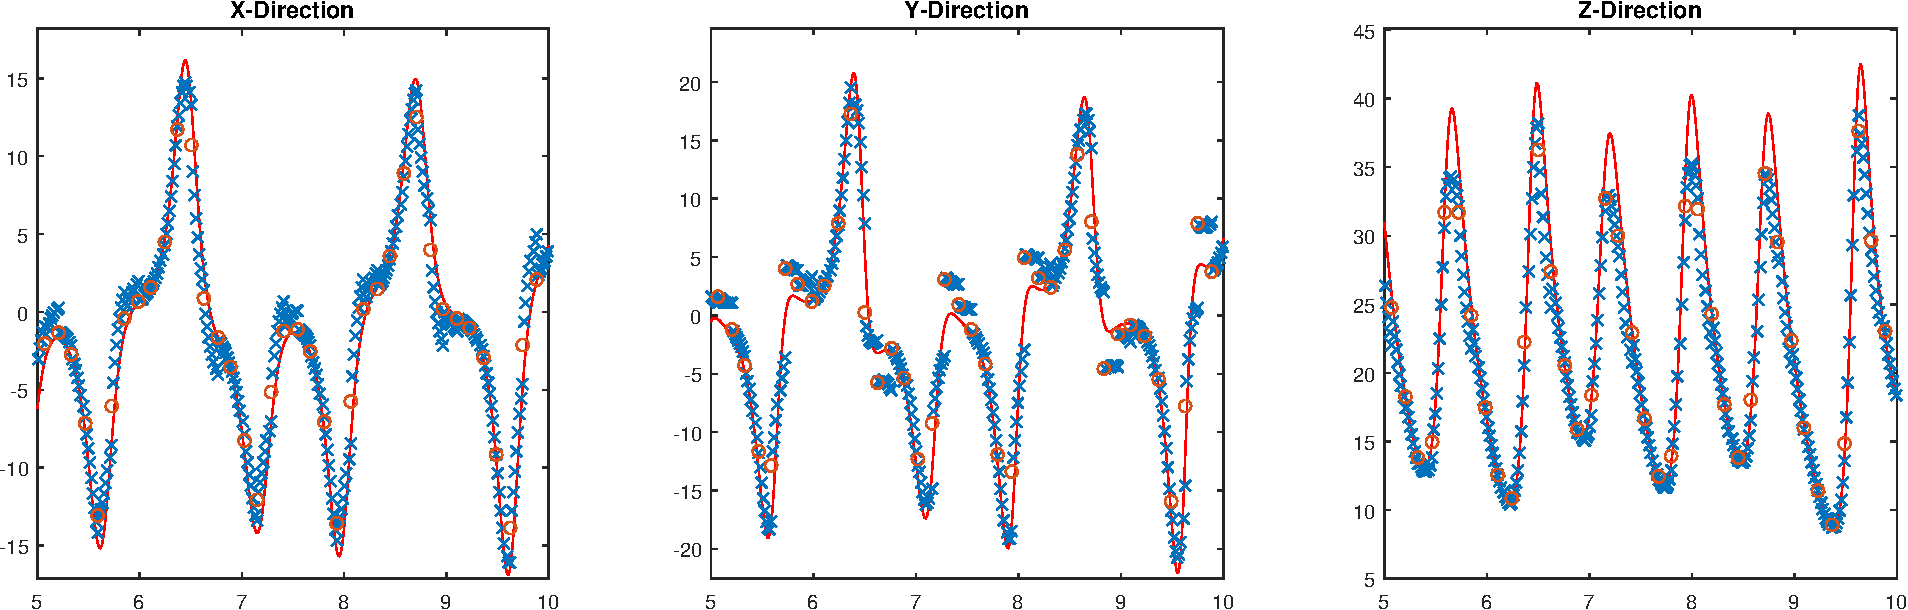
\includegraphics[width=\hsize]{kalman/figures/H1R05S5.pdf}
\caption{Messmatrix $H_{1}$ mit $S=5$ und $F=5$}
\label{kalman:H1S5}
\end{figure}

K"onnen alle Messwerte gemessen werden, aber nur als Linearkombination wie mit $H_{2}$, sind Verschleppungen von Oszillationen aus einer Achse in eine andere erkennbar. In Abbildung \ref{kalman:H2S1} ist zu erkennen, das trotz dieser Schwierigkeit, der Filter die Realit"at sehr gut vorhersagen kann. Jedoch scheint eine Verbesserung der Messgenauigkeit keine Verbesserung der Vorhersagen zu bewirken.
Auch die Messrate zu verdoppeln l"ost die Problematik nur bedingt, da nun h"aufiger kombinierte Werte gemessen werden, die um den Wert anderer Koordinaten verschoben sind. Die Simulation ist hier verl"asslicher als mit der Messmatrix $H_{1}$, trotzdem ist eine regelm"assige Referenzierung unerl"asslich. So verlief der Versuch unter allen bisher genannten Bedingungen negativ, den Fehler der Simulation st"arker zu gewichten als den Messfehler.

\begin{figure}
\centering
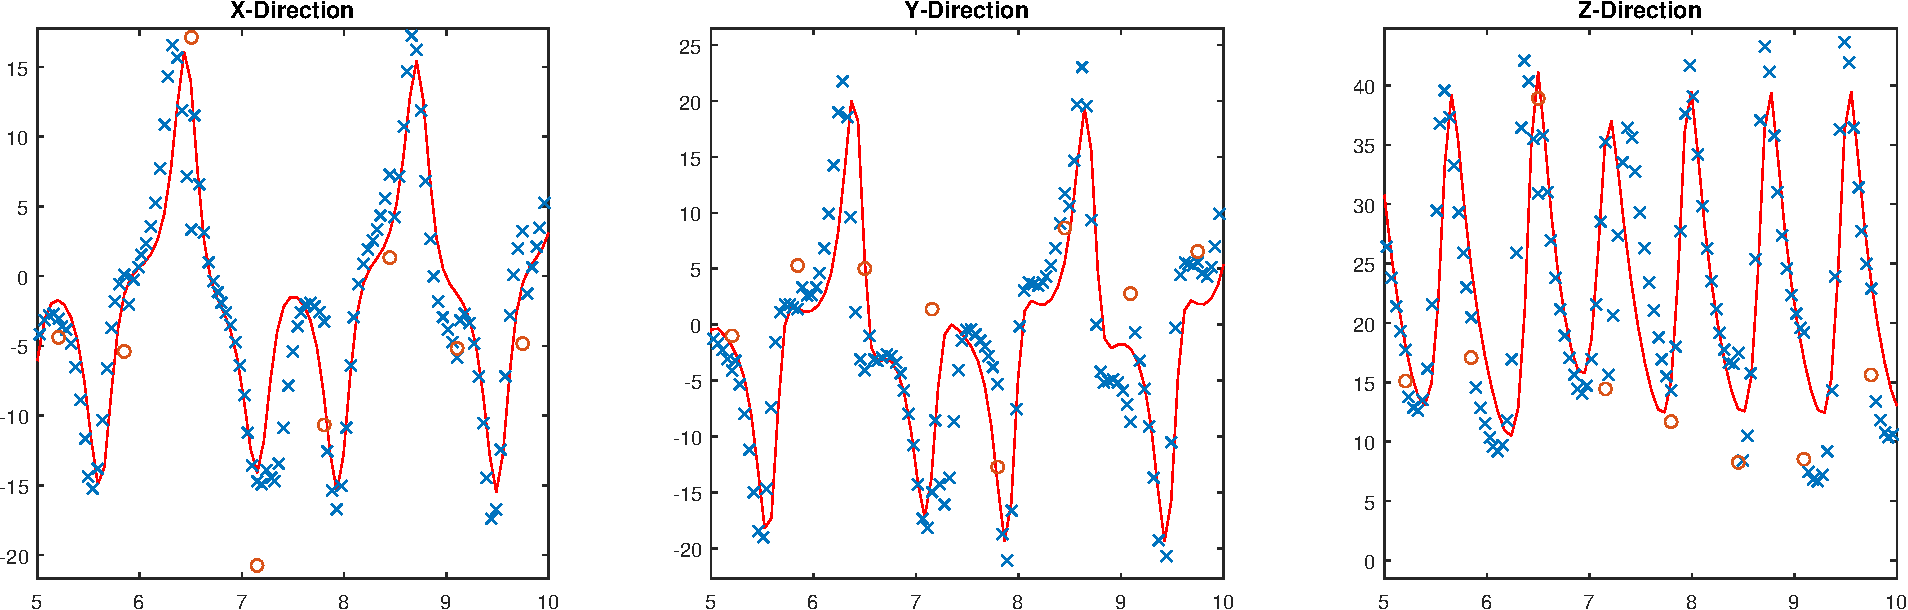
\includegraphics[width=\hsize]{kalman/figures/H2R05S1.pdf}
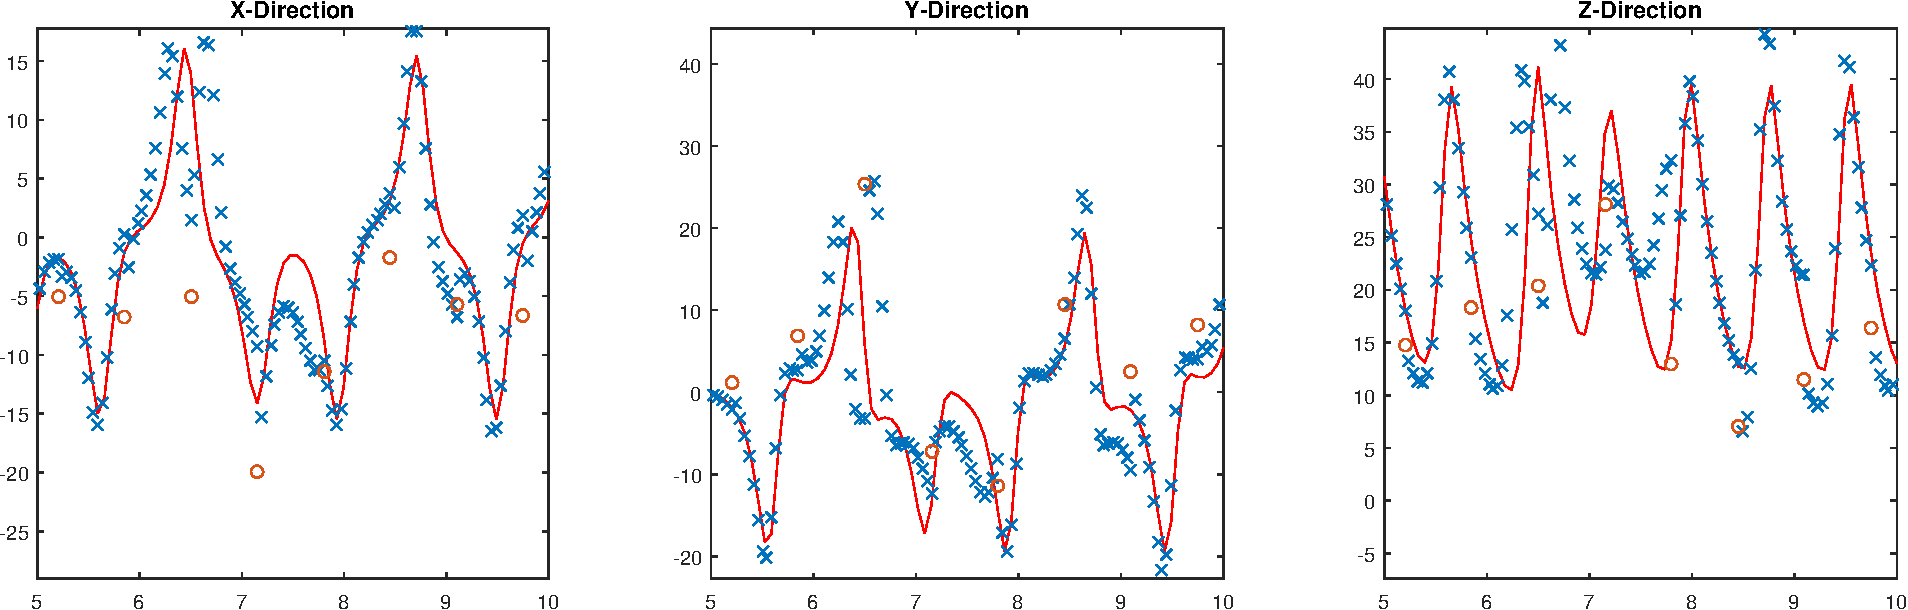
\includegraphics[width=\hsize]{kalman/figures/H2R20S1.pdf}
\caption{Messmatrix $H_{2}$ mit $S=1$ und $F=5$ (oben) und $F=20$ (unten)}
\label{kalman:H2S1}
\end{figure}

\begin{figure}
\centering
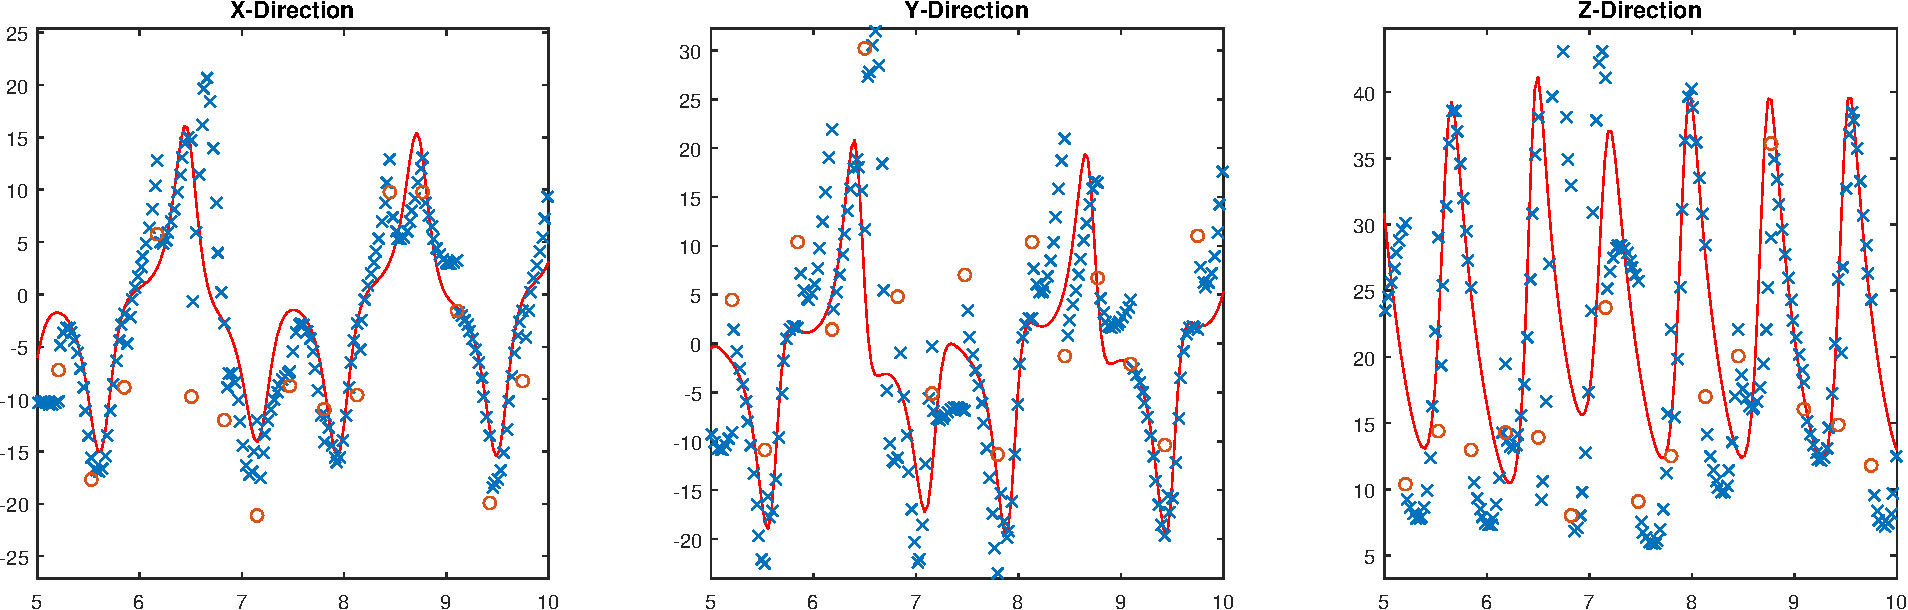
\includegraphics[width=\hsize]{kalman/figures/H2R10S2.pdf}
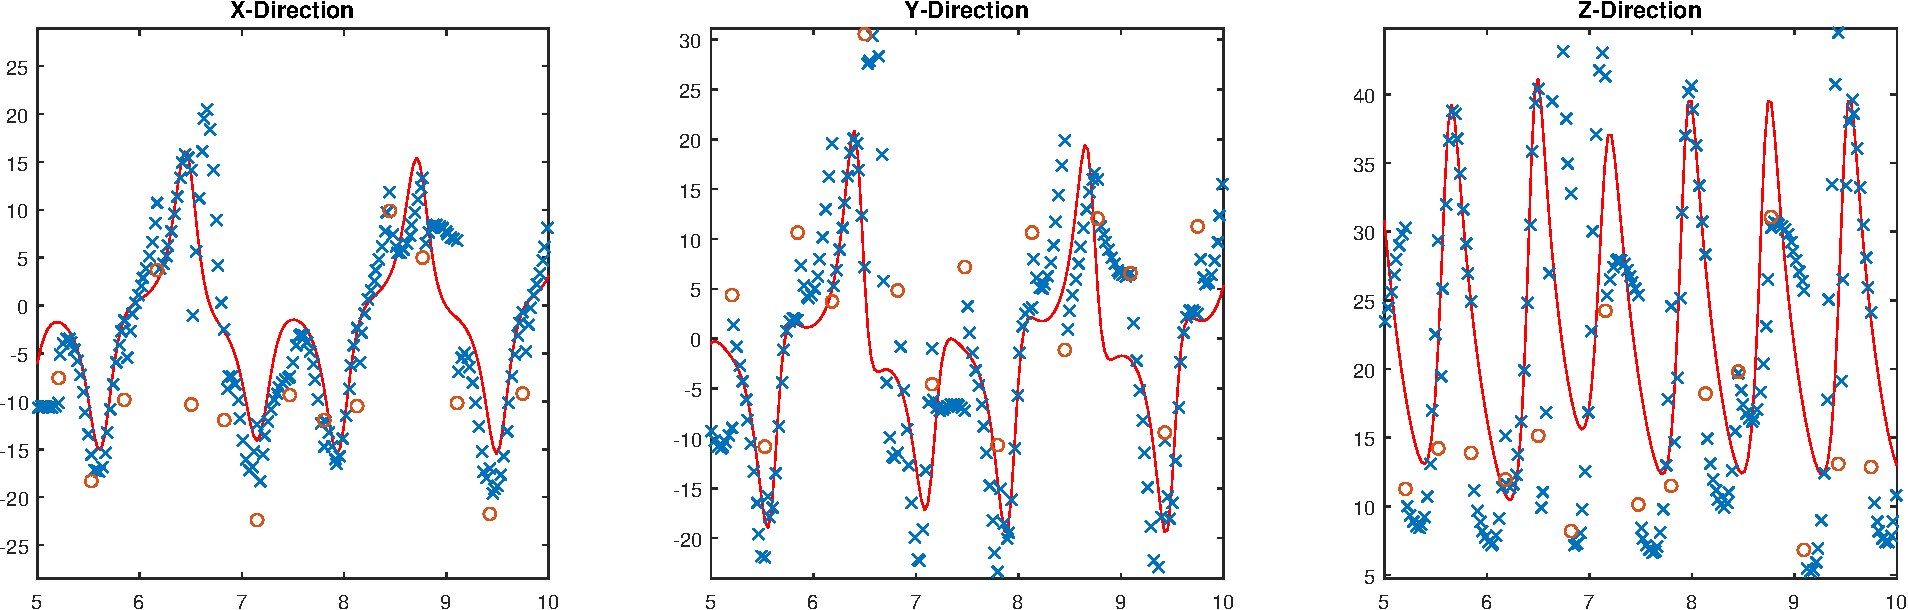
\includegraphics[width=\hsize]{kalman/figures/H2R20S2.pdf}
\caption{Messmatrix $H_{2}$ mit $S=2$ und $F=10$ (oben) und $F=20$ (unten)}
\label{kalman:H2S2}
\end{figure}

Wird die Messkadenz noch einmal wie in Abbildung \ref{kalman:H2S5} erh"oht, scheinen einzig die Werte in $X-$ und $Z$-Richtung verl"asslichere Vorhersagen und bessere gefilterte Daten zu liefern. Der $Y$-Wert und deren Simulationen zeigen h"aufig gar in die falsche Richtung. Dies kann darauf zur"uckgef"uhrt werden, dass in der Gleichung f"ur $Y$ alle drei Koordinaten Einfluss nehmen und so eine richtige Korrektur erschwert wird. Aufgrund der resultierenden Abweichung folgt dann eine schlechte Vorhersage.

\begin{figure}
\centering
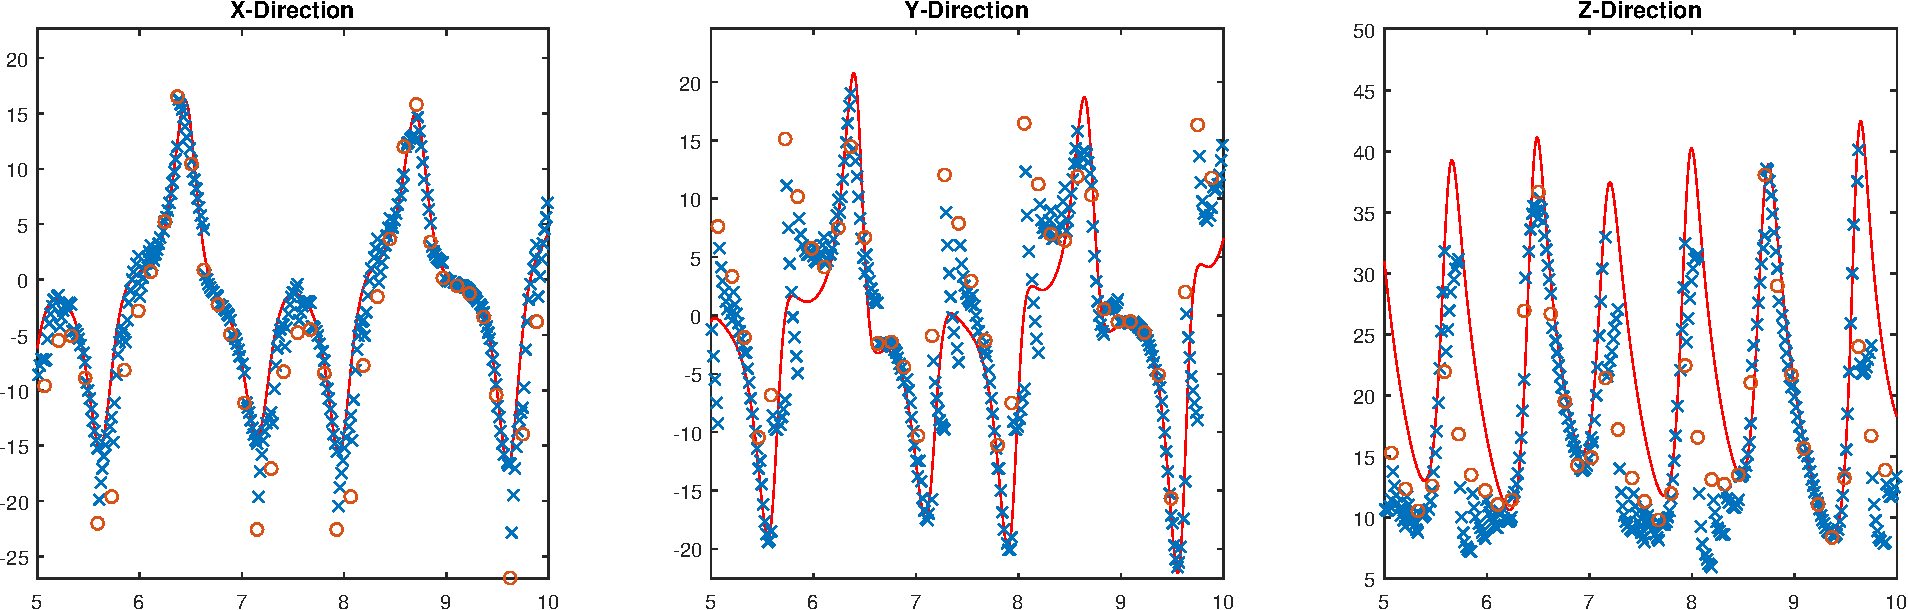
\includegraphics[width=\hsize]{kalman/figures/H2R05S5.pdf}
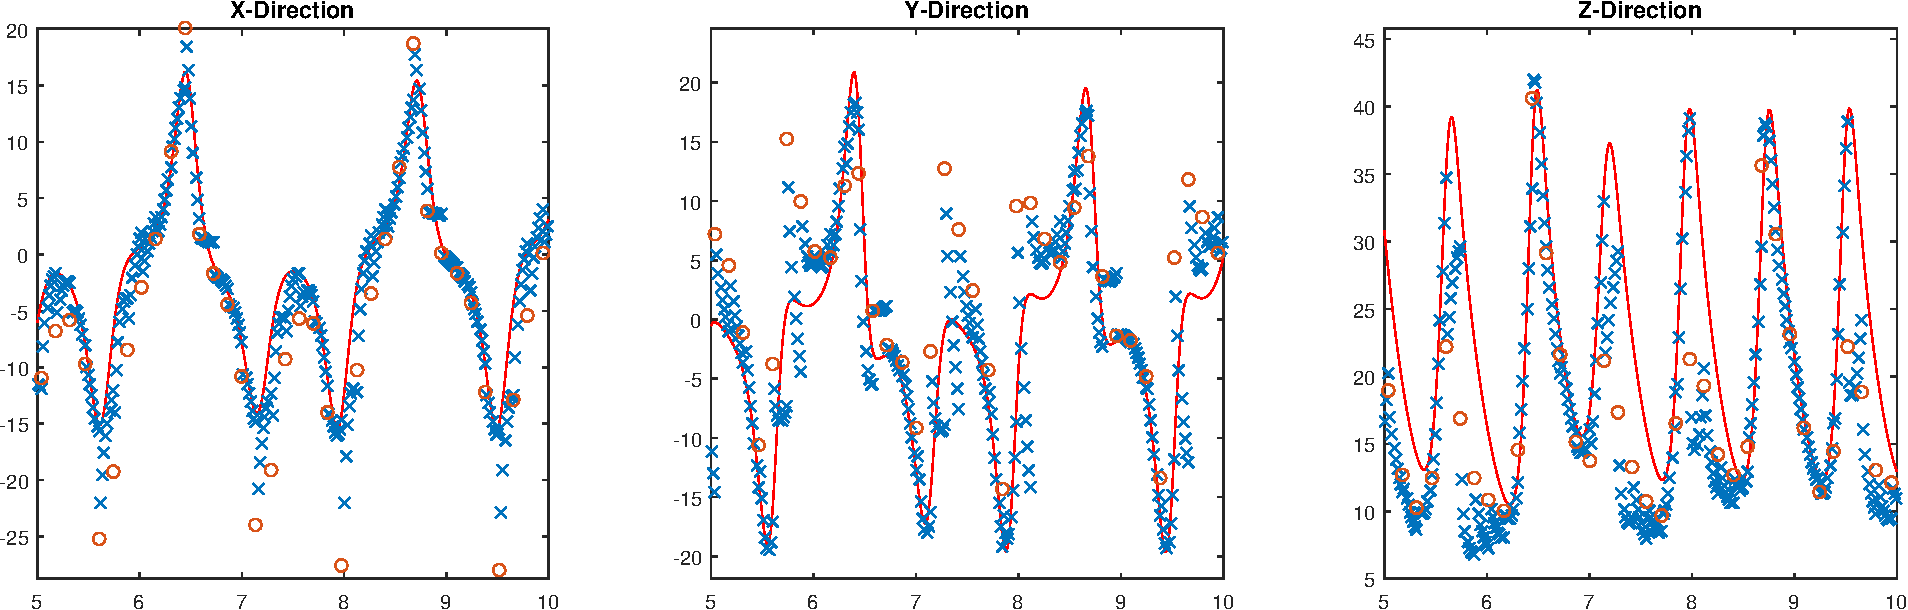
\includegraphics[width=\hsize]{kalman/figures/H2R10S5.pdf}
\caption{Messmatrix $H_{2}$ mit $S=5$ und $F=5$ (oben) und $F=10$ (unten)}
\label{kalman:H2S5}
\end{figure}

\subsection{Unvollst"andig erfassbares System}
\rhead{Unvollst"andig erfassberes System}
Nun zu den unvollst"andig erfassbaren Systemen mit den Messmatritzen 
\[H_{3}=\begin{pmatrix}
1 & 0 & 0 \\ 
0 & 1 & 0 \\ 
\end{pmatrix} 
\text{ und }
H_{4}=\begin{pmatrix}
1 & 0 & 0 \\ 
0 & 0 & 1
\end{pmatrix}
\text{.}
\]
Gem"ass der rechten Seite des Lorenz Modells \eqref{kalman:lm63} ist bekannt, dass alle drei Werte von einander abh"angen, und so folglich alle zur Verf"ugung stehen m"ussten. In Abbildung \ref{kalman:H3} der Versuch, mit verschiedenen $F$ und $S$ der Situation trotzdem Herr zu werden. Erst im mittleren Bild mit $S=2$ und $F=20$ ist die Anzahl der richtig vorhergesagten Werten, abgesehen von den Werten f"ur $Z$, in der "Uberzahl. Wird die Messkadenz weiter erh"oht, folgen die Simulationen gut der Realit"at, wobei die Schwierigkeit erneut bei den Werten f"ur $Y$ liegt, da $Z$ Werte komplett auf Simulationen beruhen. Das "uberhaupt eine Rekonstruktion m"oglich ist, ist der Tatsache geschuldet, dass die $Z$-Achse keine Informationen "uber das Chaos des Systems enth"alt, daher ob die Konvektionszelle mit oder gegen den Uhrzeigersinn str"omt. Dies ist sowohl in den diversen $Z$-Ansichten zu erkennen, wo die Werte mit ann"ahernd gleichbleibender Oszillation und Amplitude vorkommen, sowie in der Abbildung \ref{kalman:zview} mit der Sicht in die $XY$-Ebene.
Folglich k"onnen hier mit einer h"oheren Messkadenz bessere Ergebnisse erzielt werden, als wenn die Messgenauigkeit erh"oht wird.

\begin{figure}
\centering
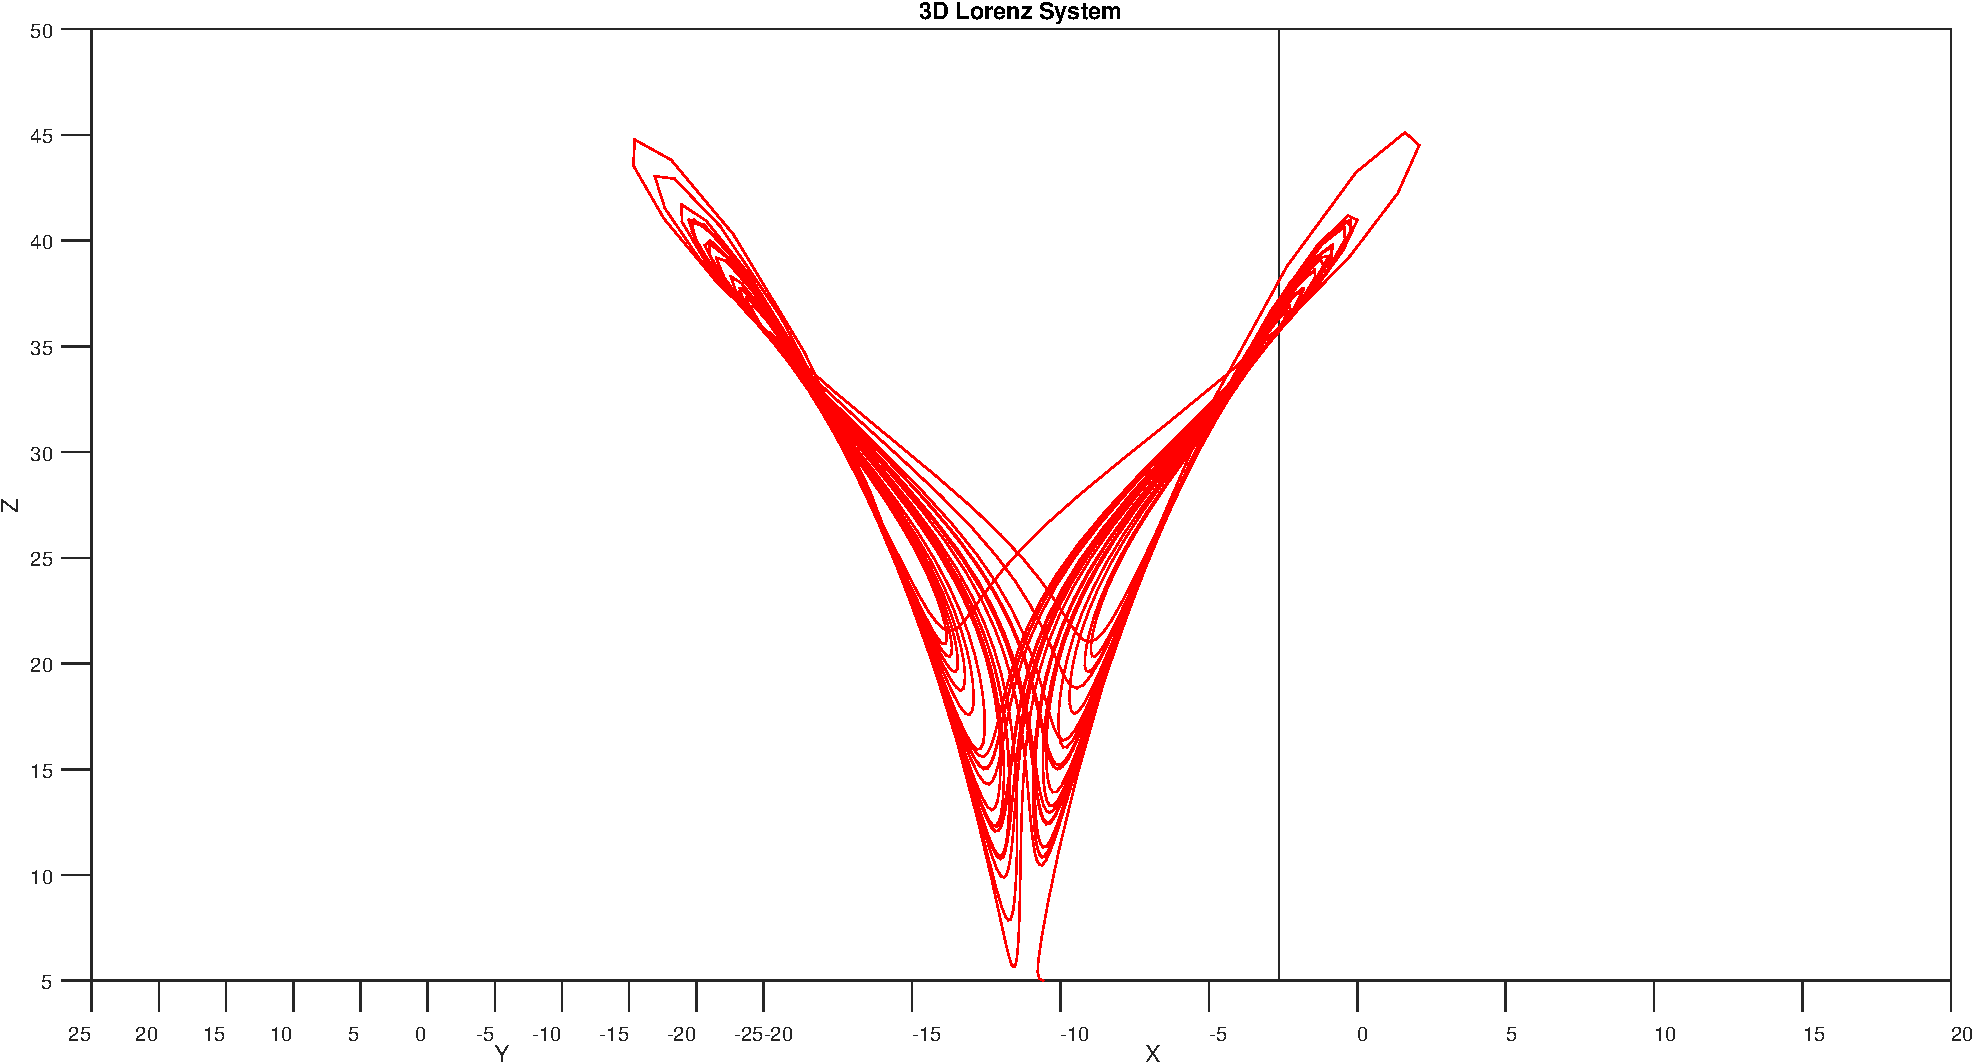
\includegraphics[width=\hsize]{kalman/figures/zview.pdf}
\caption{3-D Lorenz System mit Sicht auf $Z$-Achse}
\label{kalman:zview}
\end{figure}

\begin{figure}
\centering
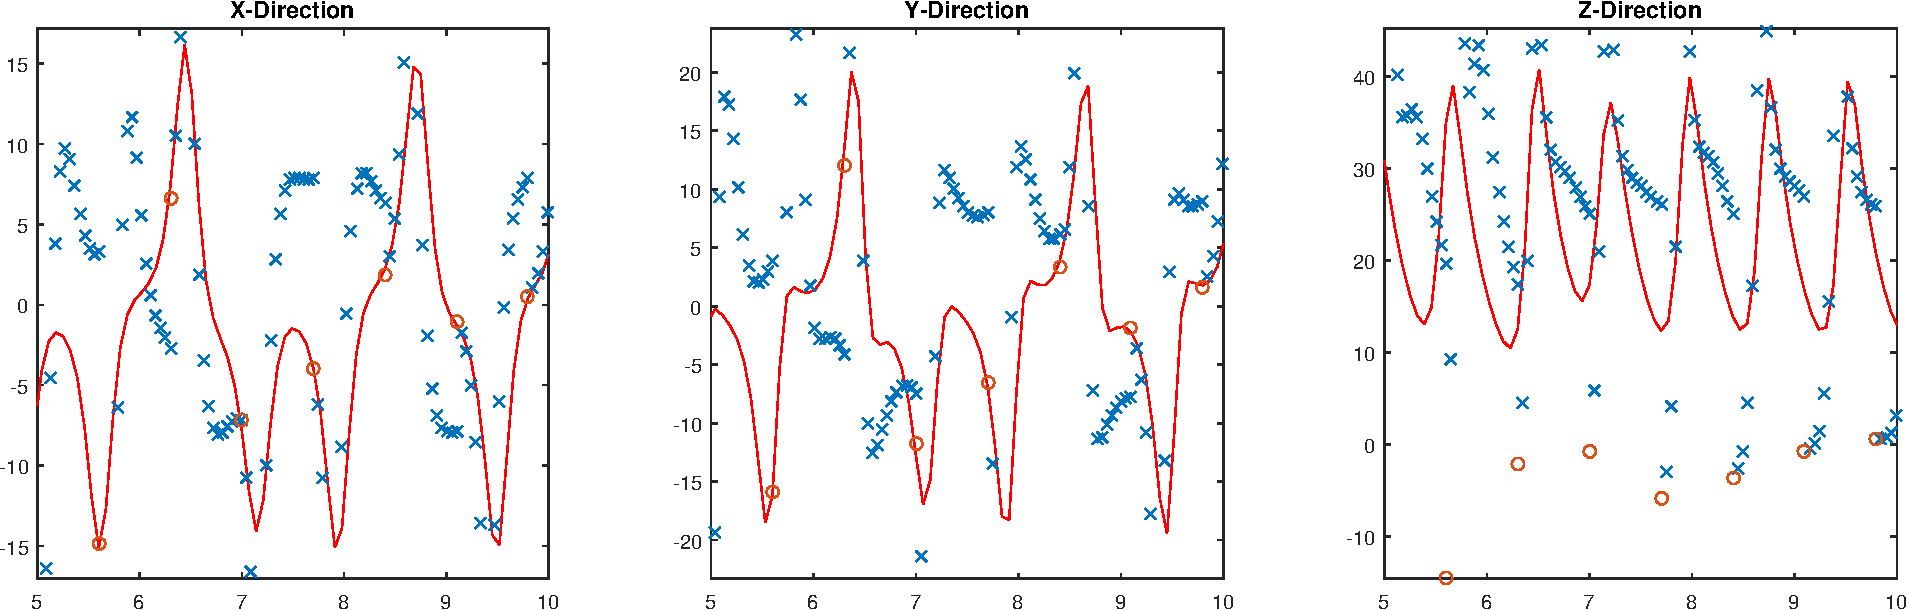
\includegraphics[width=\hsize]{kalman/figures/H3R10S1.pdf}
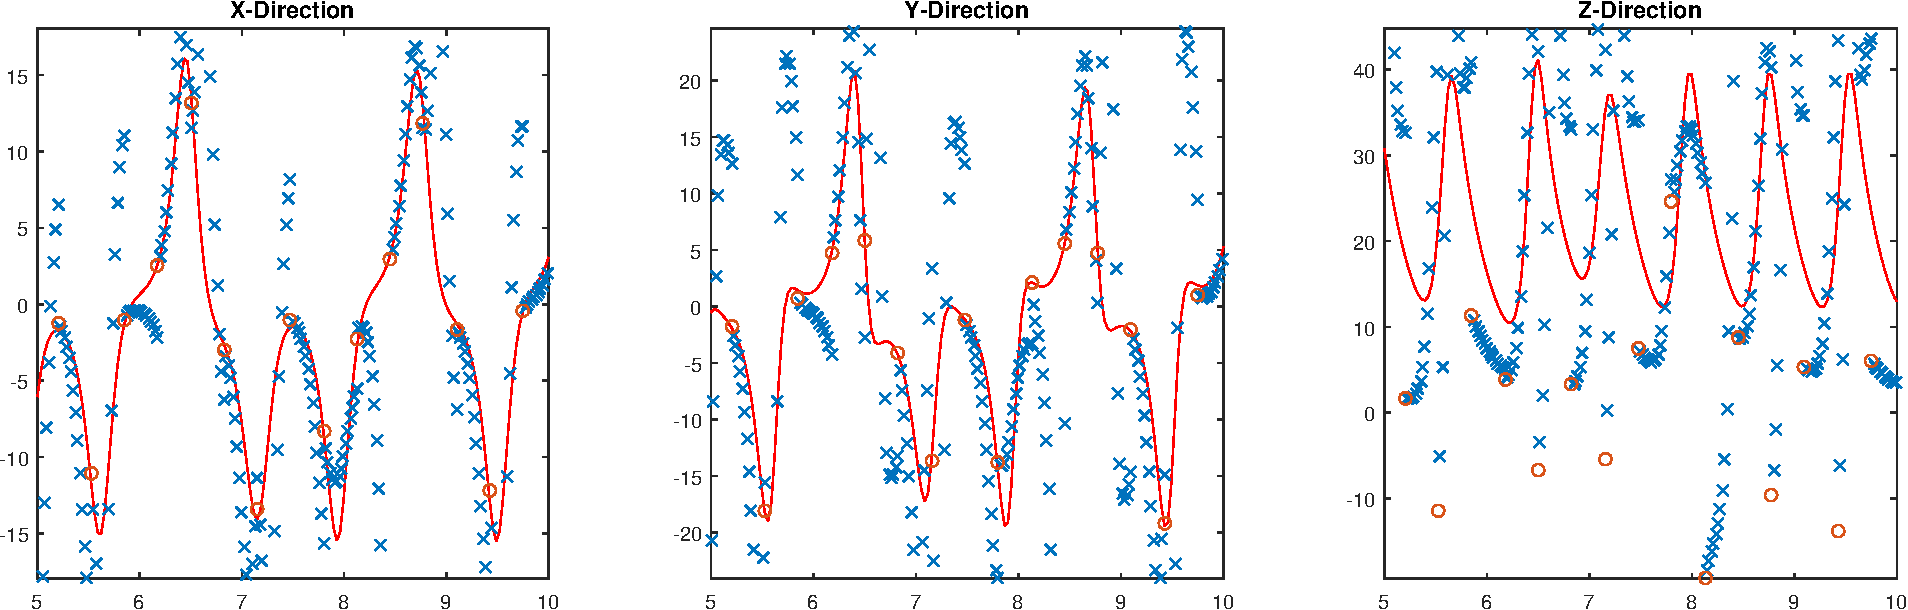
\includegraphics[width=\hsize]{kalman/figures/H3R20S2.pdf}
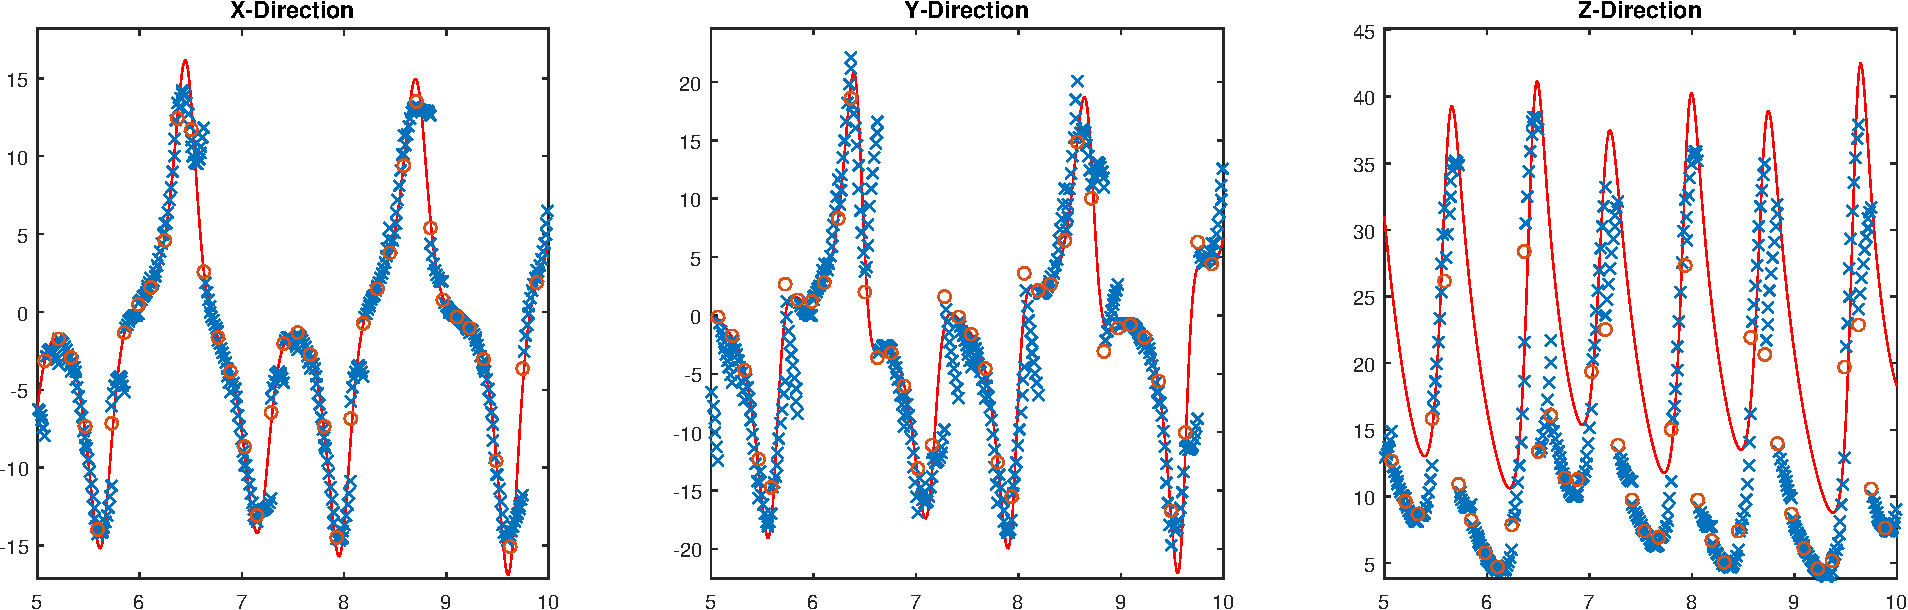
\includegraphics[width=\hsize]{kalman/figures/H3R05S5.pdf}
\caption{Messmatrix $H_{3}$ mit $S=1$, $F=10$ (oben), $S=2$ und $F=20$ (mitte) und $S=5$ und $F=5$ (unten)}
\label{kalman:H3}
\end{figure}

Liegen wie mit $H_{4}$ in Abbildung \ref{kalman:H4} lediglich Werte f"ur $X$ und $Z$ vor, reicht dies nicht mehr f"ur eine Rekonstruktion der Realit"at. Die Simulationen liegen, abgesehen von den $Z$ Werten, "ofters daneben, als dass sie die Drehrichtung richtig angeben. Eine Erh"ohung der Messkadenz oder genaueres Messen hilft nicht, die Vorhersagen zu verbessern. Dies deshalb, da das $Y$ relevante Informationen "uber das Gesamtsystem enth"alt.
Da die Messwerte f"ur $X$ und $Z$ zur Verf"ugung stehen, korrigiert der Filter diese trotzdem richtig.
Die Rekonstruktion der $Z$ Werte scheint unter Umst"anden m"oglich zu sein, da kein chaotisches Verhalten vorliegt und daf"ur weniger Werte zur Verf"ugung stehen m"ussen.

\begin{figure}
\centering
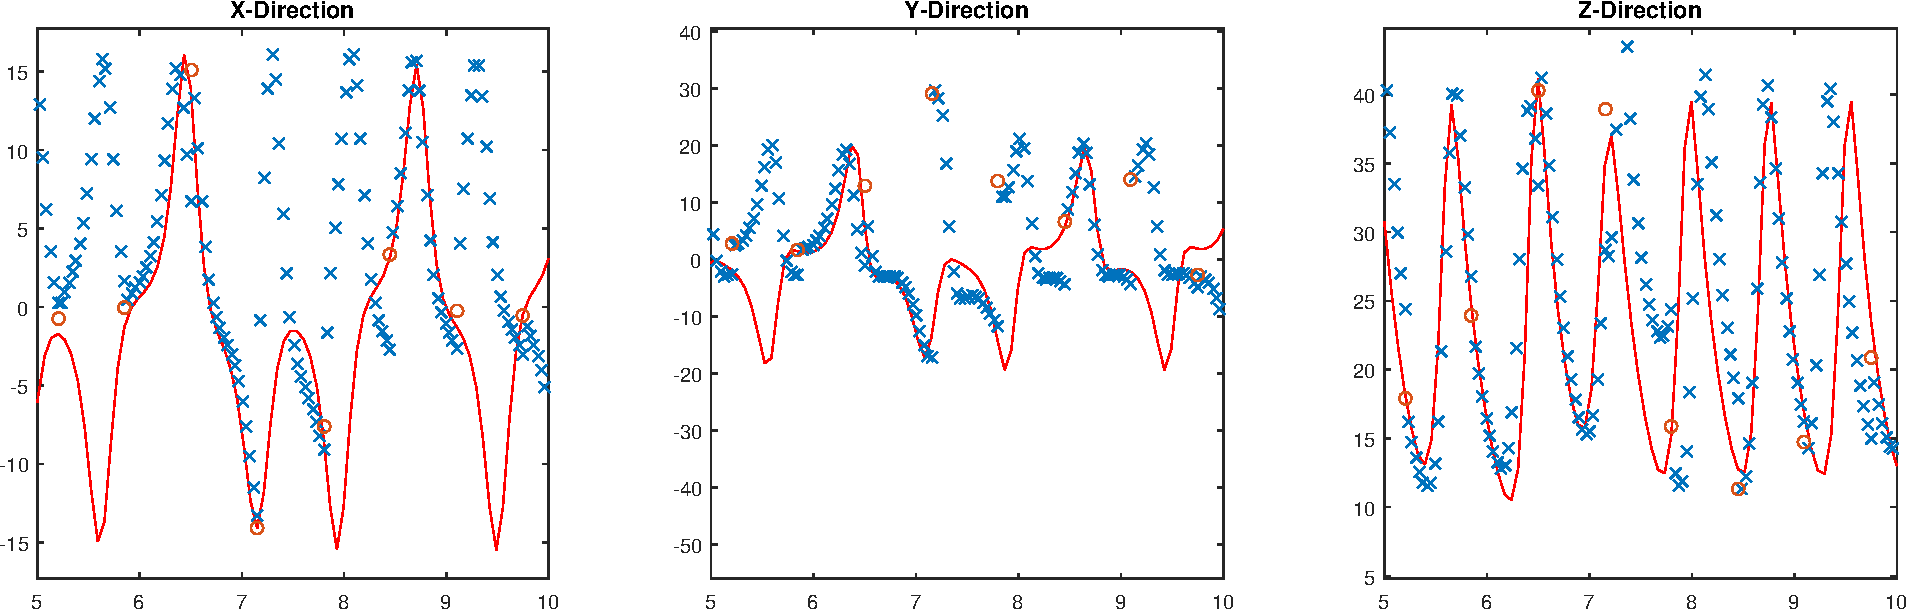
\includegraphics[width=\hsize]{kalman/figures/H4R10S1.pdf}
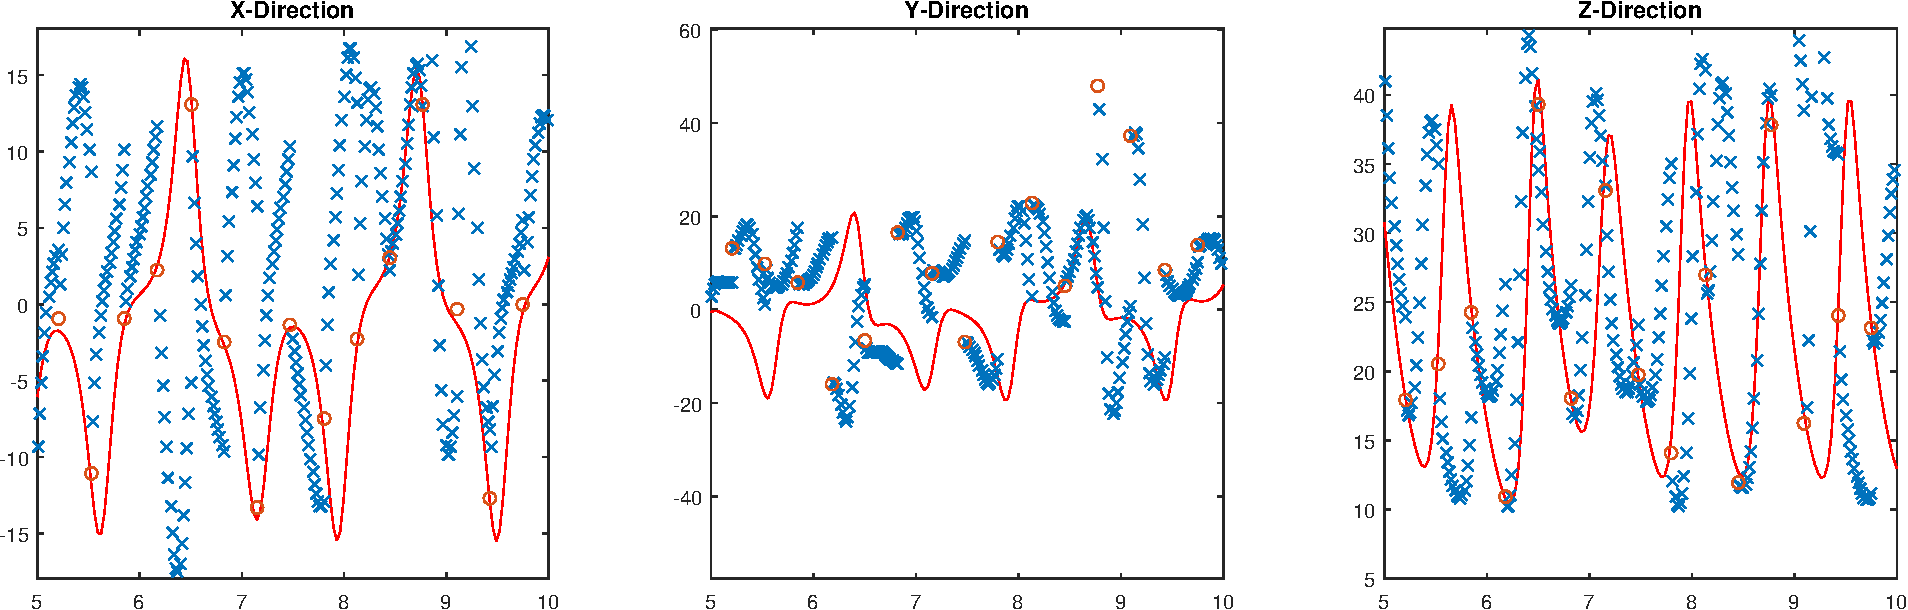
\includegraphics[width=\hsize]{kalman/figures/H4R20S2.pdf}
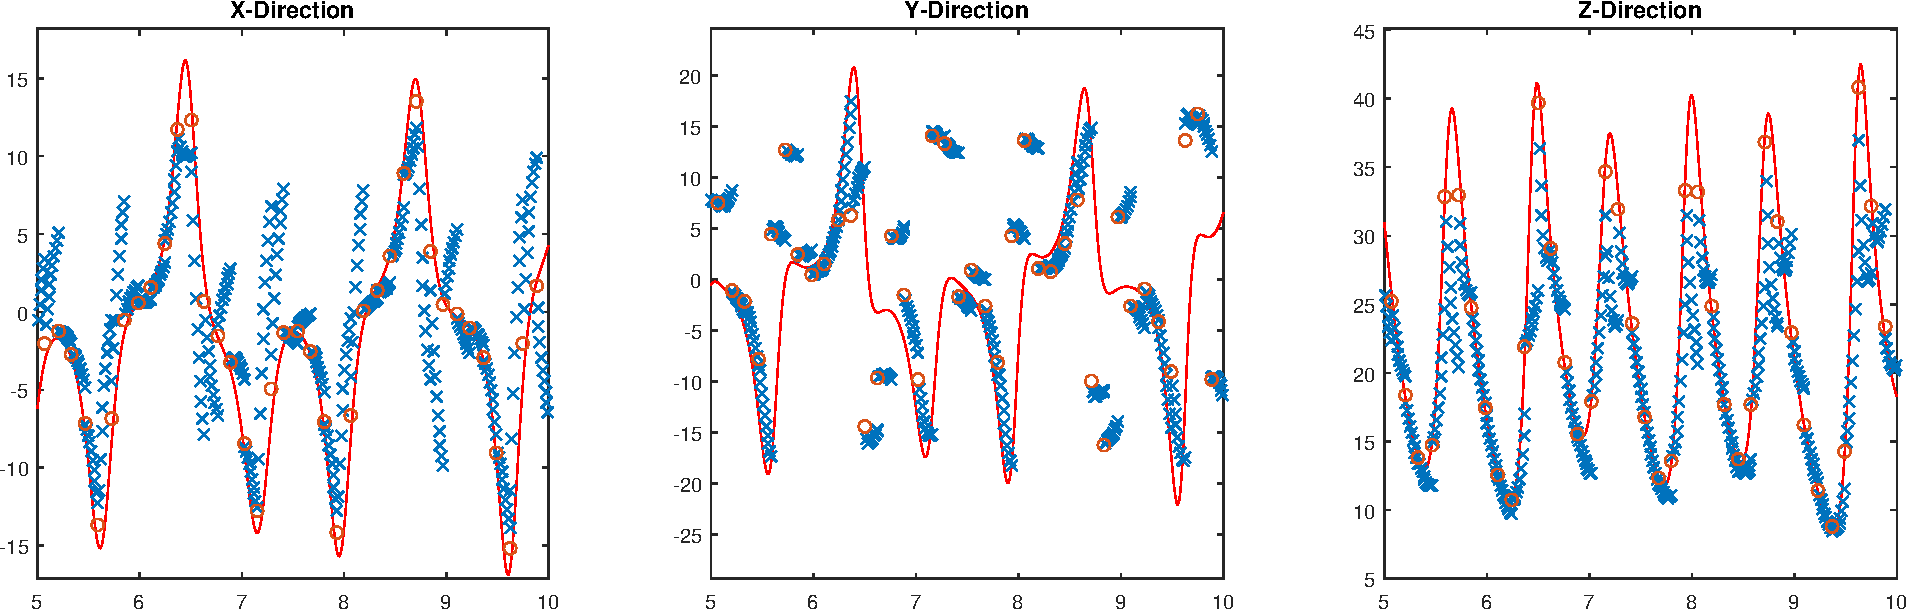
\includegraphics[width=\hsize]{kalman/figures/H4R05S5.pdf}
\caption{Messmatrix $H_{4}$ mit $S=1$ und $F=10$ (oben), $S=2$ und $F=20$ (mitte), $S=5$ und $F=5$ (unten)}
\label{kalman:H4}
\end{figure}

\section{Zusammenfassung der Erkenntnisse}
\rhead{Zusammenfassung der Erkenntnisse}
\begin{itemize}

\item
Auf eine h"ohere Messgenauigkeit kann auch zugunsten einer zeitlich besser koordinierten Messung verzichtet werden. Dies konnte erfolgreich mit der Datenassimilation gezeigt werden. Es ist aber anzunehmen, dass auch dass eine stark chaotische Komponente beinhaltet und so keine konkrete Aussage gemacht werden kann, welcher Zeitpunkt f"ur zum Beispiel eine Temperatur- oder Druckmessung optimal ist. 

\item
Eine st"arkere Gewichtung zugunsten der Simulation bringt selbst bei dieser Anwendung, wo die Realit"at mit dem Systemmodell identisch ist, keine besseren Resultate. Dies wird grunds"atzlich f"ur chaotische Systeme gelten. So m"ussen f"ur gute Resultate, beim vollst"andig erfassbaren System, die Messfehler in der gr"ossenordnung 10 bis 20-fach kleiner sein als die der Simulation, wenn nur eine Messung pro Oszillation zur Verf"ugung steht.

\item
Liegen alle Messwerte vor, aber als Linearkombination wie mit $H_{2}$, so lassen sich mit dem Kalmanfilter erfolgreiche Vorhersagen treffen. Dies jedoch, bei gleicher Messgenauigkeit und -h"aufigkeit, schlechter, als wenn alle Parameter individuell vorliegen und deutlich besser, als wenn Parameter fehlen.

\item
Eine der wichtigeren Erkenntnisse ist, das bei einem guten Abbild der Realit"at durch ein Systemmodell weniger relevante Parameter nicht zur Verf"ugung stehen m"ussen oder deren Messungen gar obsolet werden. Um zu Entscheiden welche Parameter f"ur brauchbare Datenassimilationen mit dem Kalmanfilter notwendig sind, m"ussen ein gen"ugend gutes Systemverst"andnis und Versuchsreihen vorhanden sein. Im Falle des Lorenzmodells enth"alt die $Z$-Achse wenig Informationen "uber das chaotische Verhalten der Konvektionszelle, weshalb man unter den oben genutzten Parametern auch ohne korrigierende Messung vern"unftige Vorhersagen machen kann. Hingegen sind die Werte f"ur $Y$ systemrelevant, hier werden bei h"oherer Messgenauigkeit auch bessere Ergebnisse erzielt aber eine Rekonstruktion wird durch fehlen des Wertes verunm"oglicht.

\item
Das System neigt zu extrem chaotischem Verhalten bei marginalen "Anderungen der Parameter, was eine Rekonstruktion der Werte erschwert. Dies unter anderem darum, da nicht nur das Verh"altnis der Messgenauigkeiten und die Messrate relevante Parameter sind, sondern auch der Zeitpunkt der Messung. Generell decken sich jedoch die simulierten Werte mit den theoretischen "Uberlegungen.

\end{itemize}

\printbibliography[heading=subbibliography]
\end{refsection}
